% Created 2020-08-21 sex 19:10
% Intended LaTeX compiler: pdflatex
\documentclass[11pt]{article}
\usepackage[utf8]{inputenc}
\usepackage{lmodern}
\usepackage[T1]{fontenc}
\usepackage[top=2cm, bottom=2cm, left=2cm, right=2cm]{geometry}
\usepackage{graphicx}
\usepackage{longtable}
\usepackage{float}
\usepackage{wrapfig}
\usepackage{rotating}
\usepackage[normalem]{ulem}
\usepackage{amsmath}
\usepackage{textcomp}
\usepackage{marvosym}
\usepackage{wasysym}
\usepackage{amssymb}
\usepackage{amsmath}
\usepackage[theorems, skins]{tcolorbox}
\usepackage[style=abnt,noslsn,extrayear,uniquename=init,giveninits,justify,sccite,
scbib,repeattitles,doi=false,isbn=false,url=false,maxcitenames=2,
natbib=true,backend=biber]{biblatex}
\usepackage{url}
\usepackage[linktocpage,pdfstartview=FitH,colorlinks,
linkcolor=blue,anchorcolor=blue,
citecolor=blue,filecolor=blue,menucolor=blue,urlcolor=blue]{hyperref}
\usepackage{attachfile}
\usepackage{setspace}
\usepackage{tikz}
\addbibresource{refs.bib}
\usepackage{svg, caption, multirow}
\usepackage[english]{babel}
\author{Gabriel Petrini, Lucas Teixeira}
\date{\today}
\title{Long-run effective demand and residential investment: a Sraffian supermultiplier based analysis}
\begin{document}

\maketitle
\begin{abstract}
In this paper, we build a fully specified parsimonious Sraffian supermultiplier stock-flow consistent model (SSM-SFC) with two non-capacity creating autonomous expenditure: residential investment and debt-financed consumption.
Our model represents a closed and without government economy with workers and capitalist households and only the latter are not not credit constrained.
The introduction of residential investment implies that our SSM-SFC model has two real assets: firms' productive capital and households' real estate.
The numerical simulation experiments report the main standard Sraffian supermultiplier growth models results: 
    (i) income distribution affects growth rate only during the traverse;
    (ii) autonomous expenditures alone affects long-term growth rate and;
    (iii)  utilization rate moves towards the normal one.
As a particular result, an increase of residential investment growth rate increase implies a decrease of real estate share in total real assets.
Therefore, this model introduces both housing and asset bubbles	on Sraffian supermultiplier agenda and extends the range of autonomous expenditures alternatives.

\noindent \textbf{Keywords:} Residential Investment; Sraffian supermultiplier; Asset bubble;  Stock-Flow Consistent approach.
\end{abstract}


\section{Introduction}
\label{sec:orgd83f82d}

Non-residential investment is the most scrutinized variable in demand-led growth models so that others expenditures play a secondary role \cite{brochier_macroeconomics_2017}.
A decade after the Great Recession, this is still the case for residential investment which continues to receive sparse and unsystematic attention by the literature \cites{caverzasi_stock-flow_2013}{nikolaidi_minsky_2017}.
Despite its absence in theoretical models, there is a growing empirical literature highlighting its macrodynamic relevance \cites{leamer_housing_2007}{jorda_great_2014}{fiebiger_semi-autonomous_2018}{fiebiger_trend_2017}.
In this paper, we try to fill this gap in demand-led growth agenda.


Sraffian supermultiplier growth model (SSM) establishes an important role to non-capacity creating (NCC) autonomous expenditures.
\textcite{serrano_long_1995} --- and also more recent papers \cite{freitas_growth_2015} --- presents the SSM model in a rather parsimonious way as an alternative closure within demand-led growth model agenda \cite{serrano_sraffian_2017}.
More recently, SSM has been introduced to a broader Post-Keynesian audience by \textcites{allain_tackling_2015}{lavoie_post-keynesian_2015}{lavoie_convergence_2016}.
In summary,  SSM describes a demand-led growth pattern led by NCC autonomous expenditures such as residential investment.


Different NCC autonomous expenditures have been included in this framework. 
For instance, some scholars have investigated the macroeconomic implications of both debt-financed \cites{pariboni_autonomous_2015}{fagundes_role_2017}{mandarino-2020-worker-debt} and financial wealth-financed consumption \cite{brochier_supermultiplier_2018}.
The same applies to government expenditures \cites{allain_tackling_2015}{bougrine_autonomous_2020} and exports \cite{nah_long-run_2017}.
Nevertheless, residential investment --- another NCC autonomous expenditure --- has been systematically neglected. 
One way to include residential investment with the SSM model is through houses' own interest rate proposed by \textcite{teixeira_crescimento_2015}.
This particular real interest rate is the relevant one for house investors (households) and allow us to include asset bubble in a SSM-friendly framework.



In this paper, we include residential investment into the Sraffian supermultiplier model within a Stock-Flow Consistent framework. 
In Section \ref{sec:empirical} we introduce the so-called houses own interest rate and some residential investment related stylized facts.
Section \ref{sec:Review} reviews heterodox growth models with NCC autonomous expenditures and highlights the lack of residential investment as an autonomous expenditure.
In Section \ref{sec:Model} we present our SSM-SFC model  with two real assets: firms' capital and household' real estate. 
Section \ref{sec:runs} evaluates both short-run and fully-adjusted position equilibria in order to access the consequences of residential investment inclusion on stock-flow consistent ratios.
Next, in Section \ref{sec:Experiments}, we evaluate both traverse and steady-state dynamics through numerical simulations.
The experiments are: decrease in wage-share (Section \ref{sec:Exp1}); increase in real estate inflation (Section \ref{sec:Exp2}); and an increase in interest rate \ref{sec:Exp3}).
In this same Section, we also plug houses own interest rate observed data for the U.S. (from 1992 to 2019) in order to compare our simulations' results  with recent housing bubble episode.
Section \ref{sec:Conclusion} offers some concluding remarks while Appendix \ref{append:Solution} provides the analytical solution in order to assess stability condition and Appendix \ref{append:Data} presents simulation's parameters and baseline values.


\section{Empirical Motivation}
\label{sec:orgdc59f79}
\label{sec:empirical}



A current trend among empirical research on demand-led growth is about the role of NCC autonomous expenditures.
\textcite{freitas_pattern_2013} present a growth accounting decomposition and report the relevance of those expenditures in explaining Brazilian GDP growth between 1970 and 2005. \textcite{braga_investment_2018} shows evidence that economic growth and non-residential investment are explained by NCC autonomous expenditures in Brazilian economy from 1962 to 2015. For the U.S., \textcite{girardi_long-run_2016} show that NCC autonomous expenditures have permanent effects on growth rate. 
\textcite{haluska_growth_2019} employ Granger-causality tests to assess the stability of the SSM for the US (1987-2017) and report a causality from NCC autonomous expenditures to the marginal propensity to invest, as expected.
Finally, \textcite{girardi_autonomous_2018} bring evidence that those expenditures determine the investment share on GDP for twenty OECD countries. 
Nevertheless, there still is a lack of studies on the role of residential investment specifically. 
Except for \textcites{green_follow_1997}{leamer_housing_2007} ---  which shows the relevance of this expenditure to US business cycle at least since the
post-war period ---, most of those studies were published after the Great Recession (2008-2009)\footnote{More precisely, Leamer \textcite[p.~8]{leamer_housing_2007} argues that the US business cycles can be characterized as follows: ``[f]irst homes, then cars, and last business equipment''.}.

\begin{figure}[htb]
    \centering
        \caption{Share of residential investment and capacity utilization during business cycles\\\centering (Dots size grow in  time)} 
    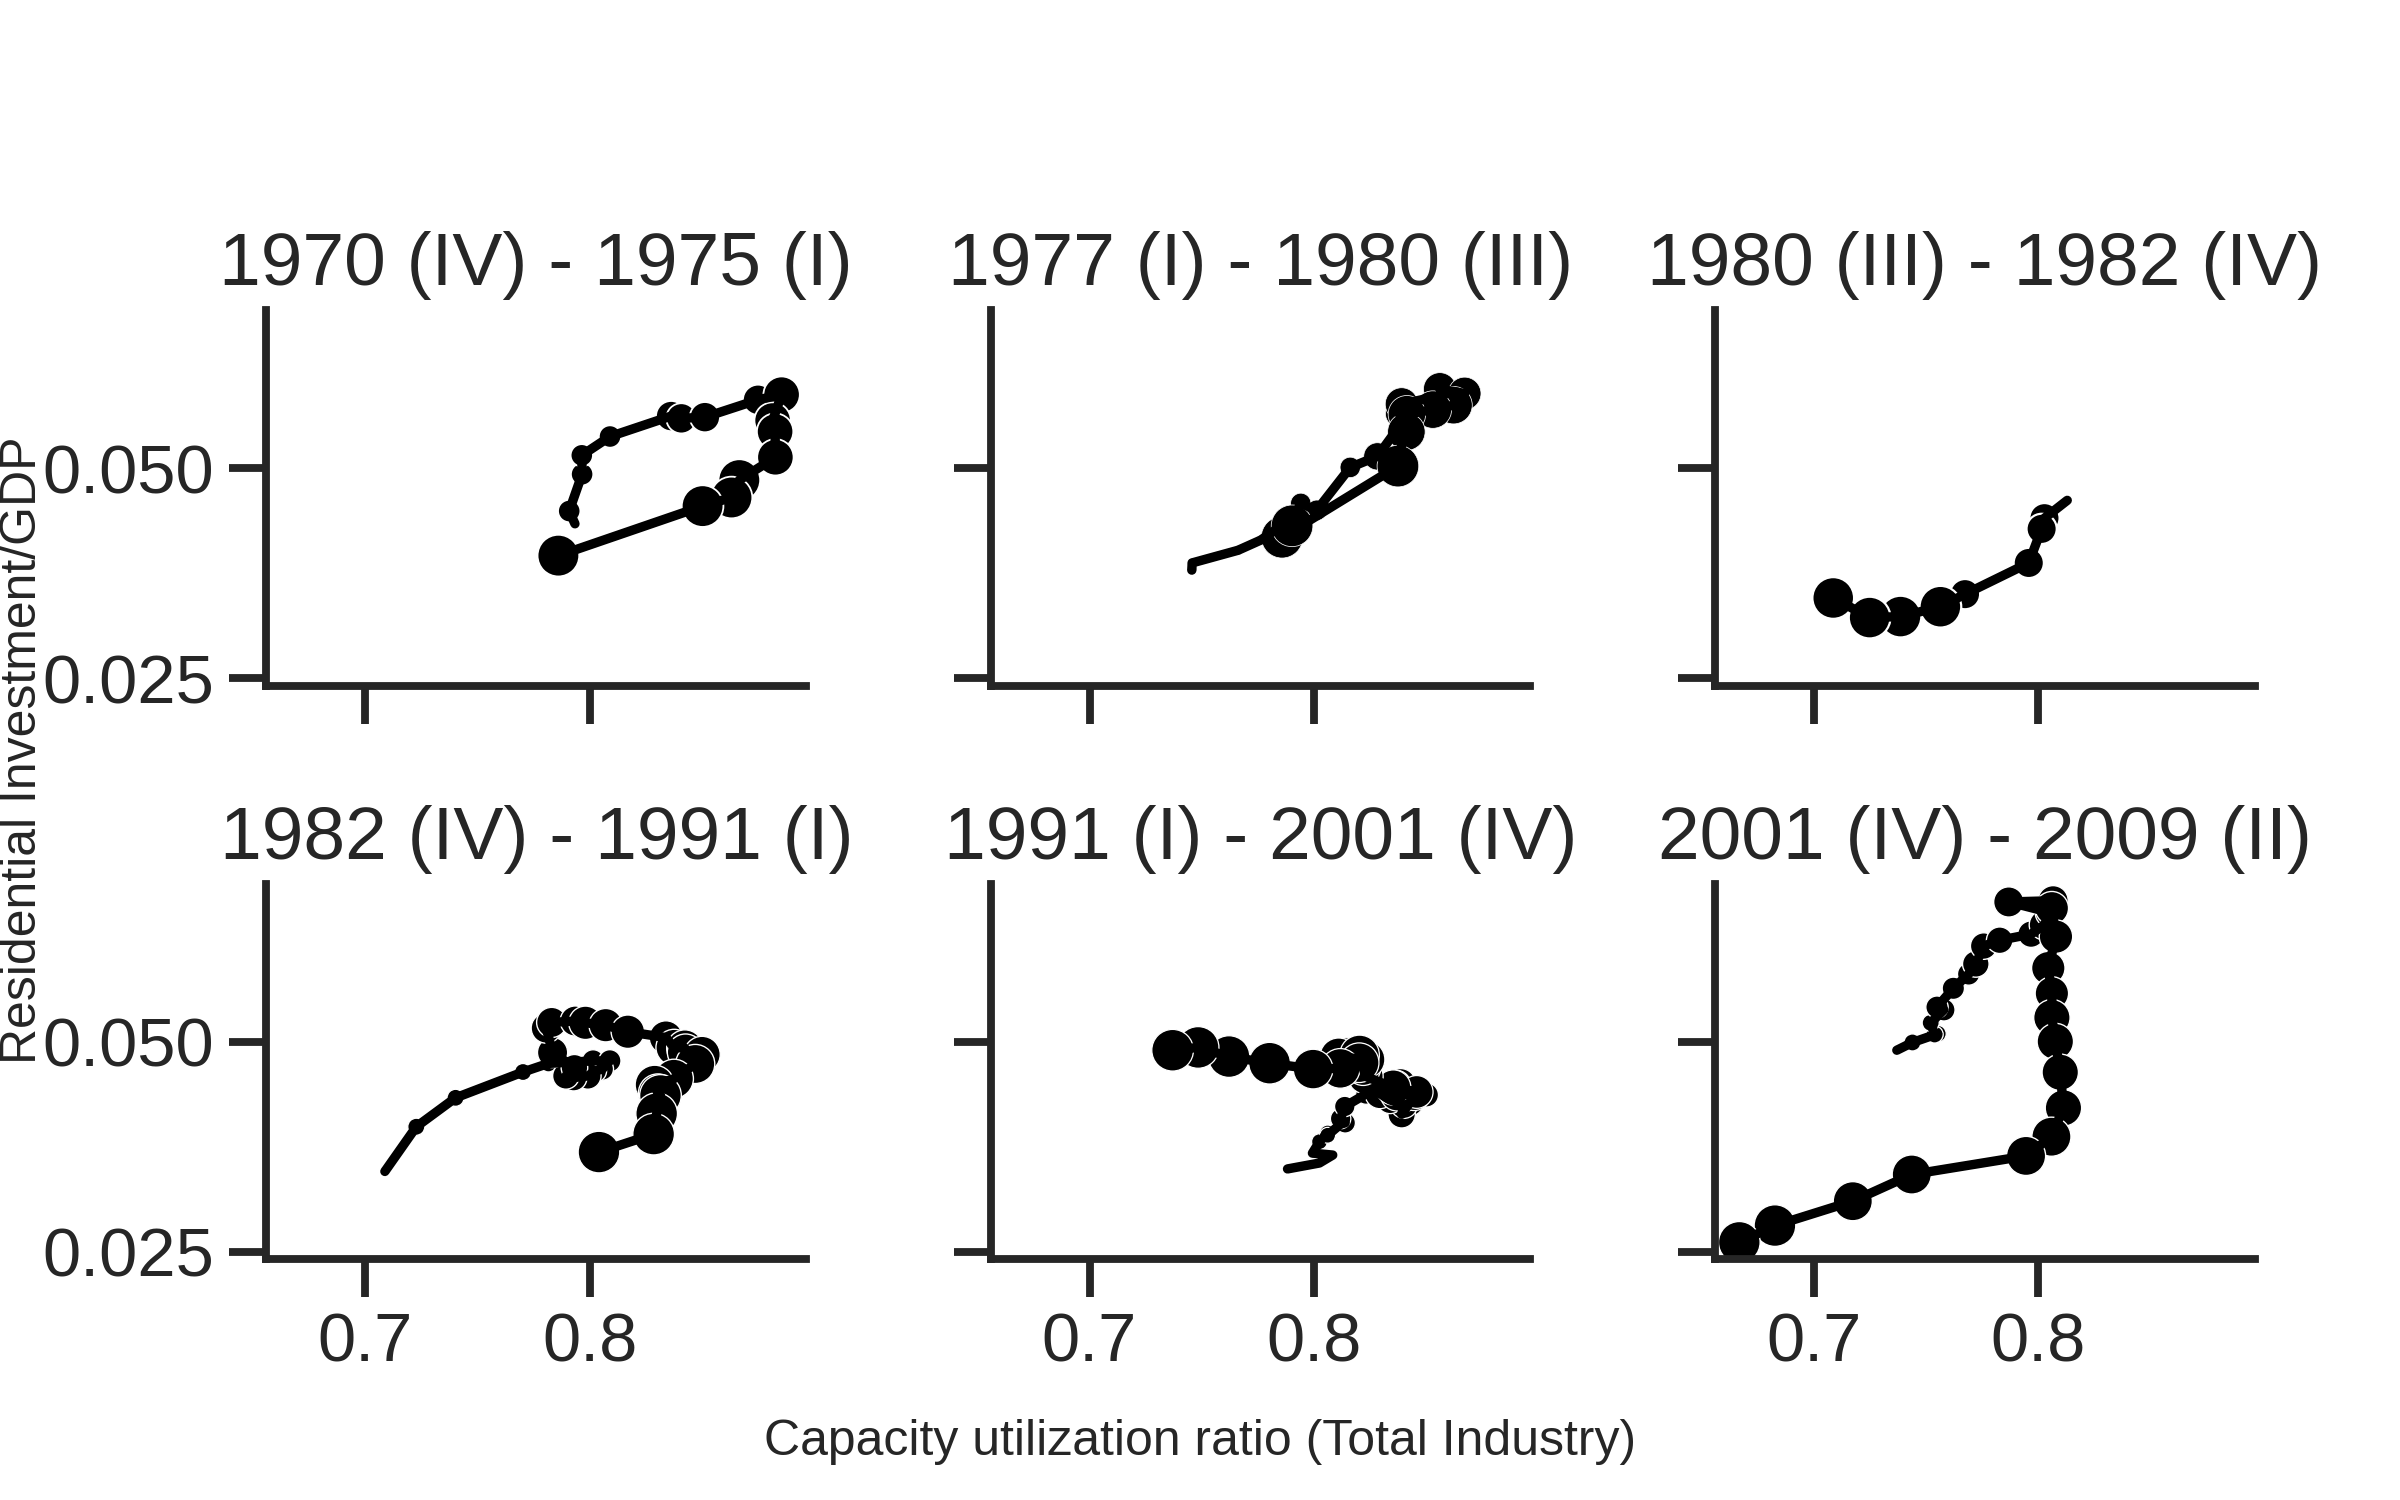
\includegraphics[width = 0.65\textwidth]{./figs/cycles.png}
    \label{fig:cycles}
    \caption*{\textbf{Source:} Federal Reserve Bank of St. Louis, authors’ elaboration.}
\end{figure}





After the Great Recession, the literature have analyzed the macroeconomic relevance of residential investment \cites{leamer_housing_2015}{fiebiger_semi-autonomous_2018}.
However, little progress has been made in understanding its theoretical determinants.
\textcite{teixeira_crescimento_2015} proposes the so-called houses own interest rate (\(own\)) in order to analyze the relation between residential investment, real estate inflation and interest rates during the U.S. housing bubble episode.
Estimated by deflating mortgages interest rate real estate inflation, this particular real interest rate is the most relevant for households since it is the real cost in real estate from buying real estate  \cite[p.~53]{teixeira_crescimento_2015}.
In short, this is the real interest rate that is relevant for house investors.
Figure \ref{propria_investo} shows how this  procedure is more adequate than a general price index deflation --- as \textcite[p.~143--6]{fair_macroeconometric_2013} does --- to describe residential investment growth rate\footnote{It is worth noting that during a housing bubble period, it is real estate inflation that governs own's interest rate dynamics.
Therefore, the lower this rate is, the greater the capital gains (in real estate) for speculating with real estate will be. This negative relation between houses own interest rate and residential investment is shown in Figure \ref{propria_investo} in which this particular real interest rate has been gradually decreased over the real estate boom (2002-5).}.
Based on this concept, \textcite{petrini_demanda_2019} estimated an econometric model for the U.S. (1992 to 2019) and presents empirical evidence that the residential investment growth rate and houses own interest rate share a common negative long-run trend.
Furthermore, \textcite{petrini_demanda_2019} also reports a unidirectional long-run causality from houses own interest rate to residential investment growth rate.


In order to depict the relation between housing and business cycle, we present Figure \ref{fig:cycles} in which each cycle is represented in a different panel\footnote{This similar reasoning can be found in \textcite{fiebiger_trend_2017}. Unlike them, we plot only residential investment without including otherhouseholds expenses financed by credit.}.
The vertical axis represents residential investment-GDP ratio and the horizontal axis represents the capacity utilization ratio  as a proxy for business cycle. Economic recovery is generally characterized by residential investment growing faster than GDP — with the 1991-2000 period being a particular case. Both residential investment share on GDP and capacity utilization increase as a consequence of this higher growth rate.
Following the Sraffian supermultiplier growth model, we conclude that increase of non-residential investment is the result of capital stock adjustment principle\footnote{\textcites{fiebiger_semi-autonomous_2018}{fiebiger_trend_2017} also report residential investment as an important determinant of business cycles. Those works associate economic instability to the behavior of (at least some) autonomous expenditures in spite of the behavior firms investment --- as it follows capital stock adjustment principle. \textcites{dejuan_hidden_2017}{teixeira_crescimento_2015} find similar results.}. This increase implies GDP to grow faster than residential investment, therefore reducing both its share on GDP and capacity utilization ratio. Finally, as a result of economic burst, capacity utilization ratio falls and the cycle ends.



\begin{figure}[htb]
	\centering
	\caption{Residential investment growth rate vs. Houses Own interest rate}
	\label{propria_investo}
	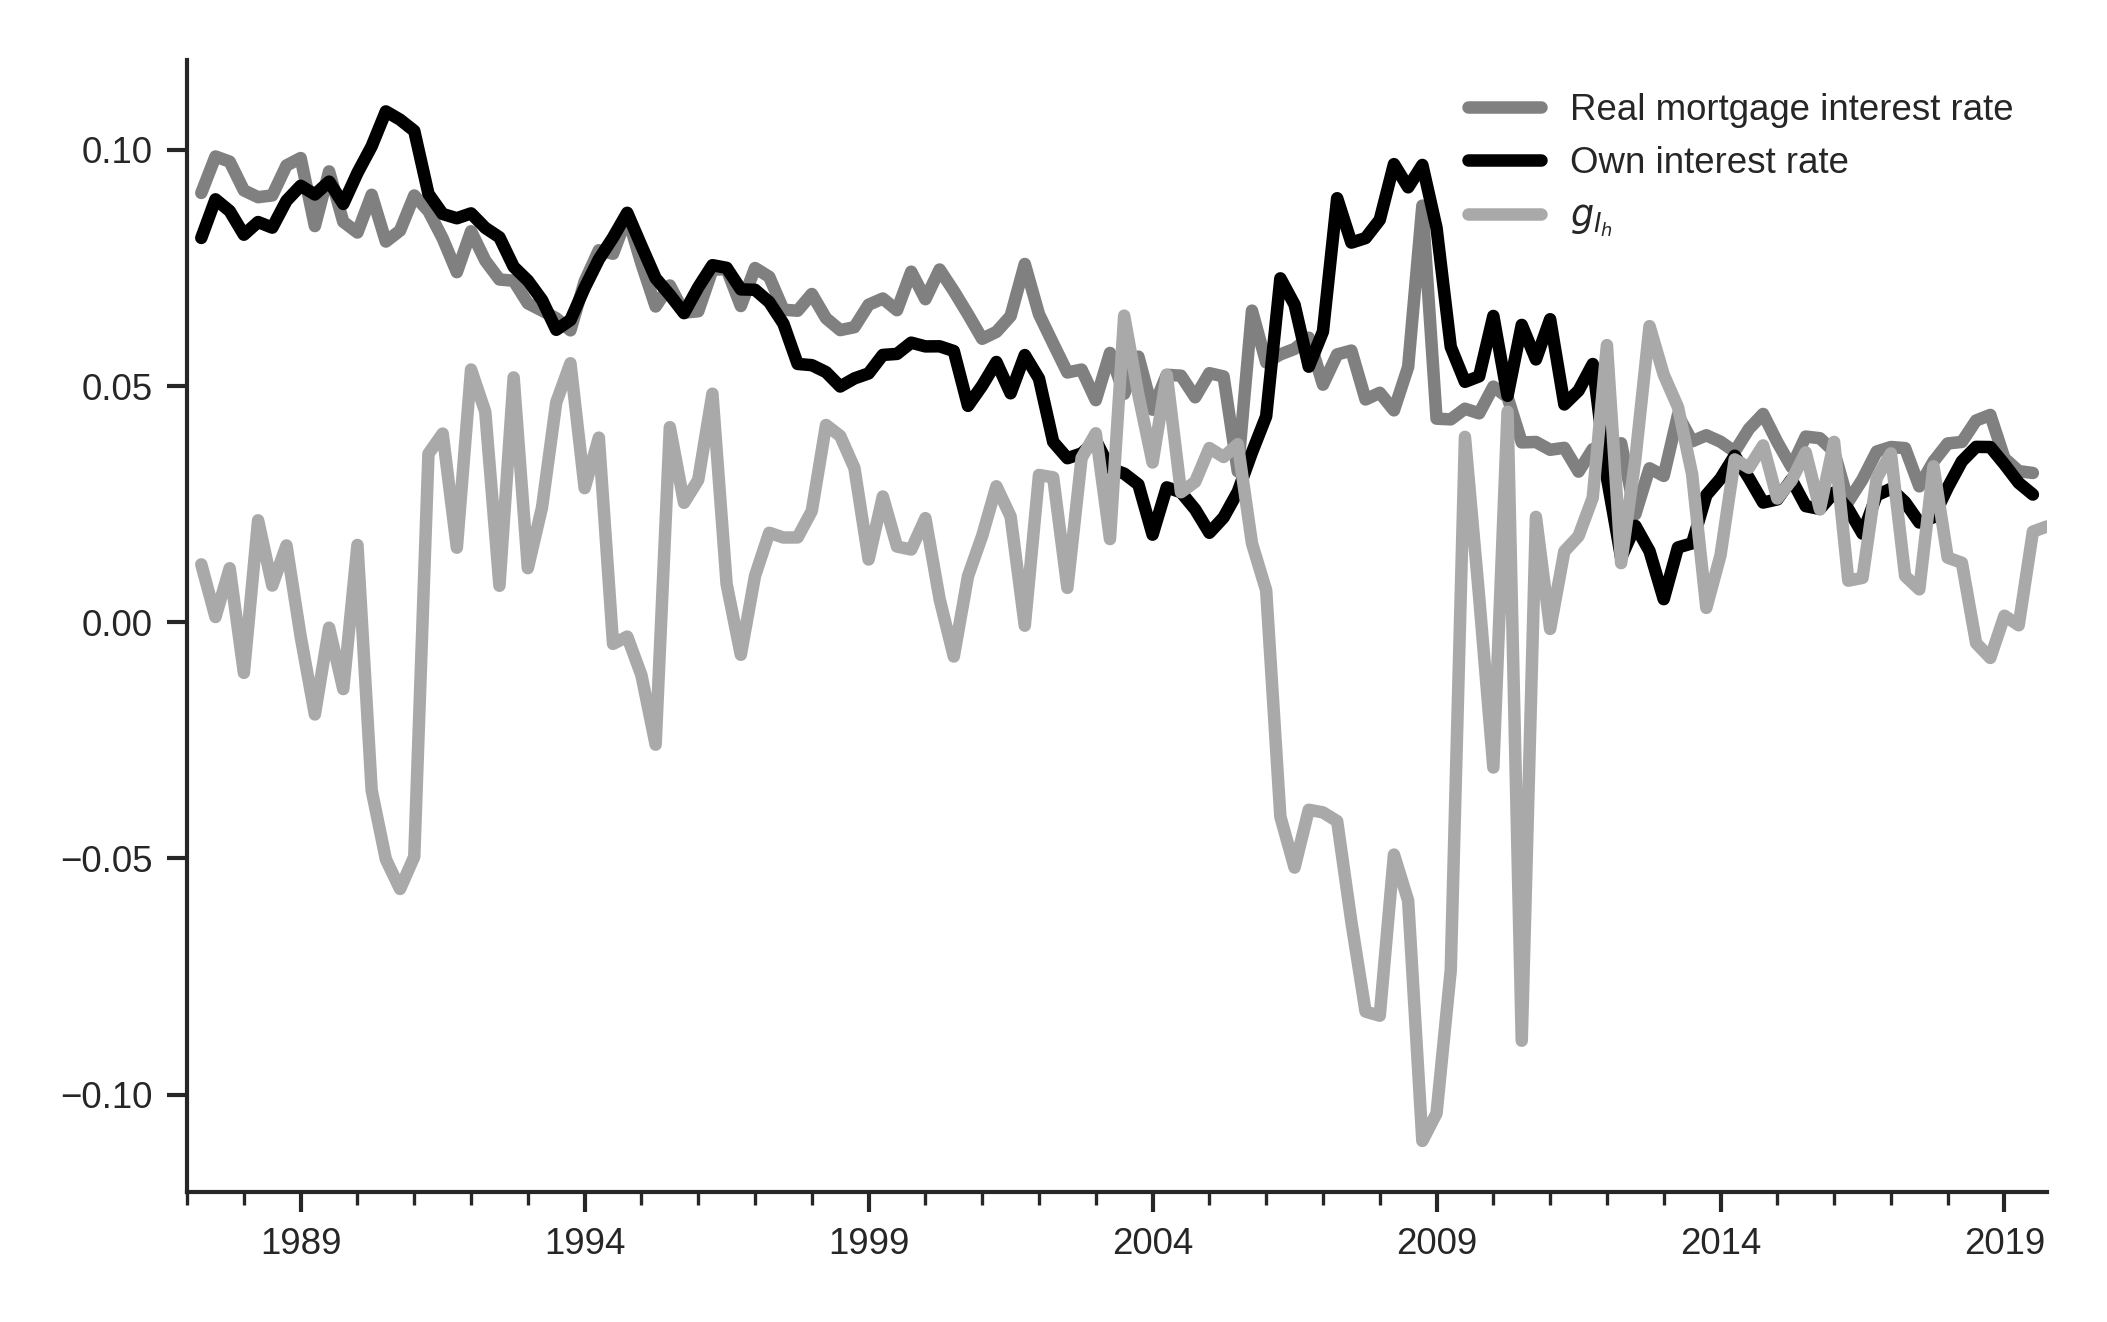
\includegraphics[width=.8\textwidth]{./figs/Own_gI}
	\caption*{\textbf{Source:} U.S. Bureau of Economic Analysis, Authors' elaboration}
\end{figure}




There is also an indirect relation between residential investment and durables goods consumption. Real estate constitutes a significant portion of household wealth so houses serves as collateral to borrowing \cite{teixeira_uma_2011}. 
As a consequence of U.S. institutional arrangement, households could increase their indebtedness as house
prices went up (see Figure \ref{fig:debt}) as a way to ``make'' capital gains without selling their houses during the 2000s housing bubble \cite{teixeira_crescimento_2015,hay_failure_2013}. 
The relation between households indebtedness and real estate inflation also describes the increasing gap between assets and liabilities in the course of the Great Recession\footnote{This co-movement results from the housing prices burst (post-2005) and  the insensitivity of households’ financial commitments. In other words, real estate (assets) has a market value while debt (liabilities) has a contractual one, thus, households net worth decreases
onset of the subprime crisis.}. 

\begin{figure}[htb]
    \centering
        \caption{Household debt and House prices\\\centering (Jan/2000 = 100)} 
    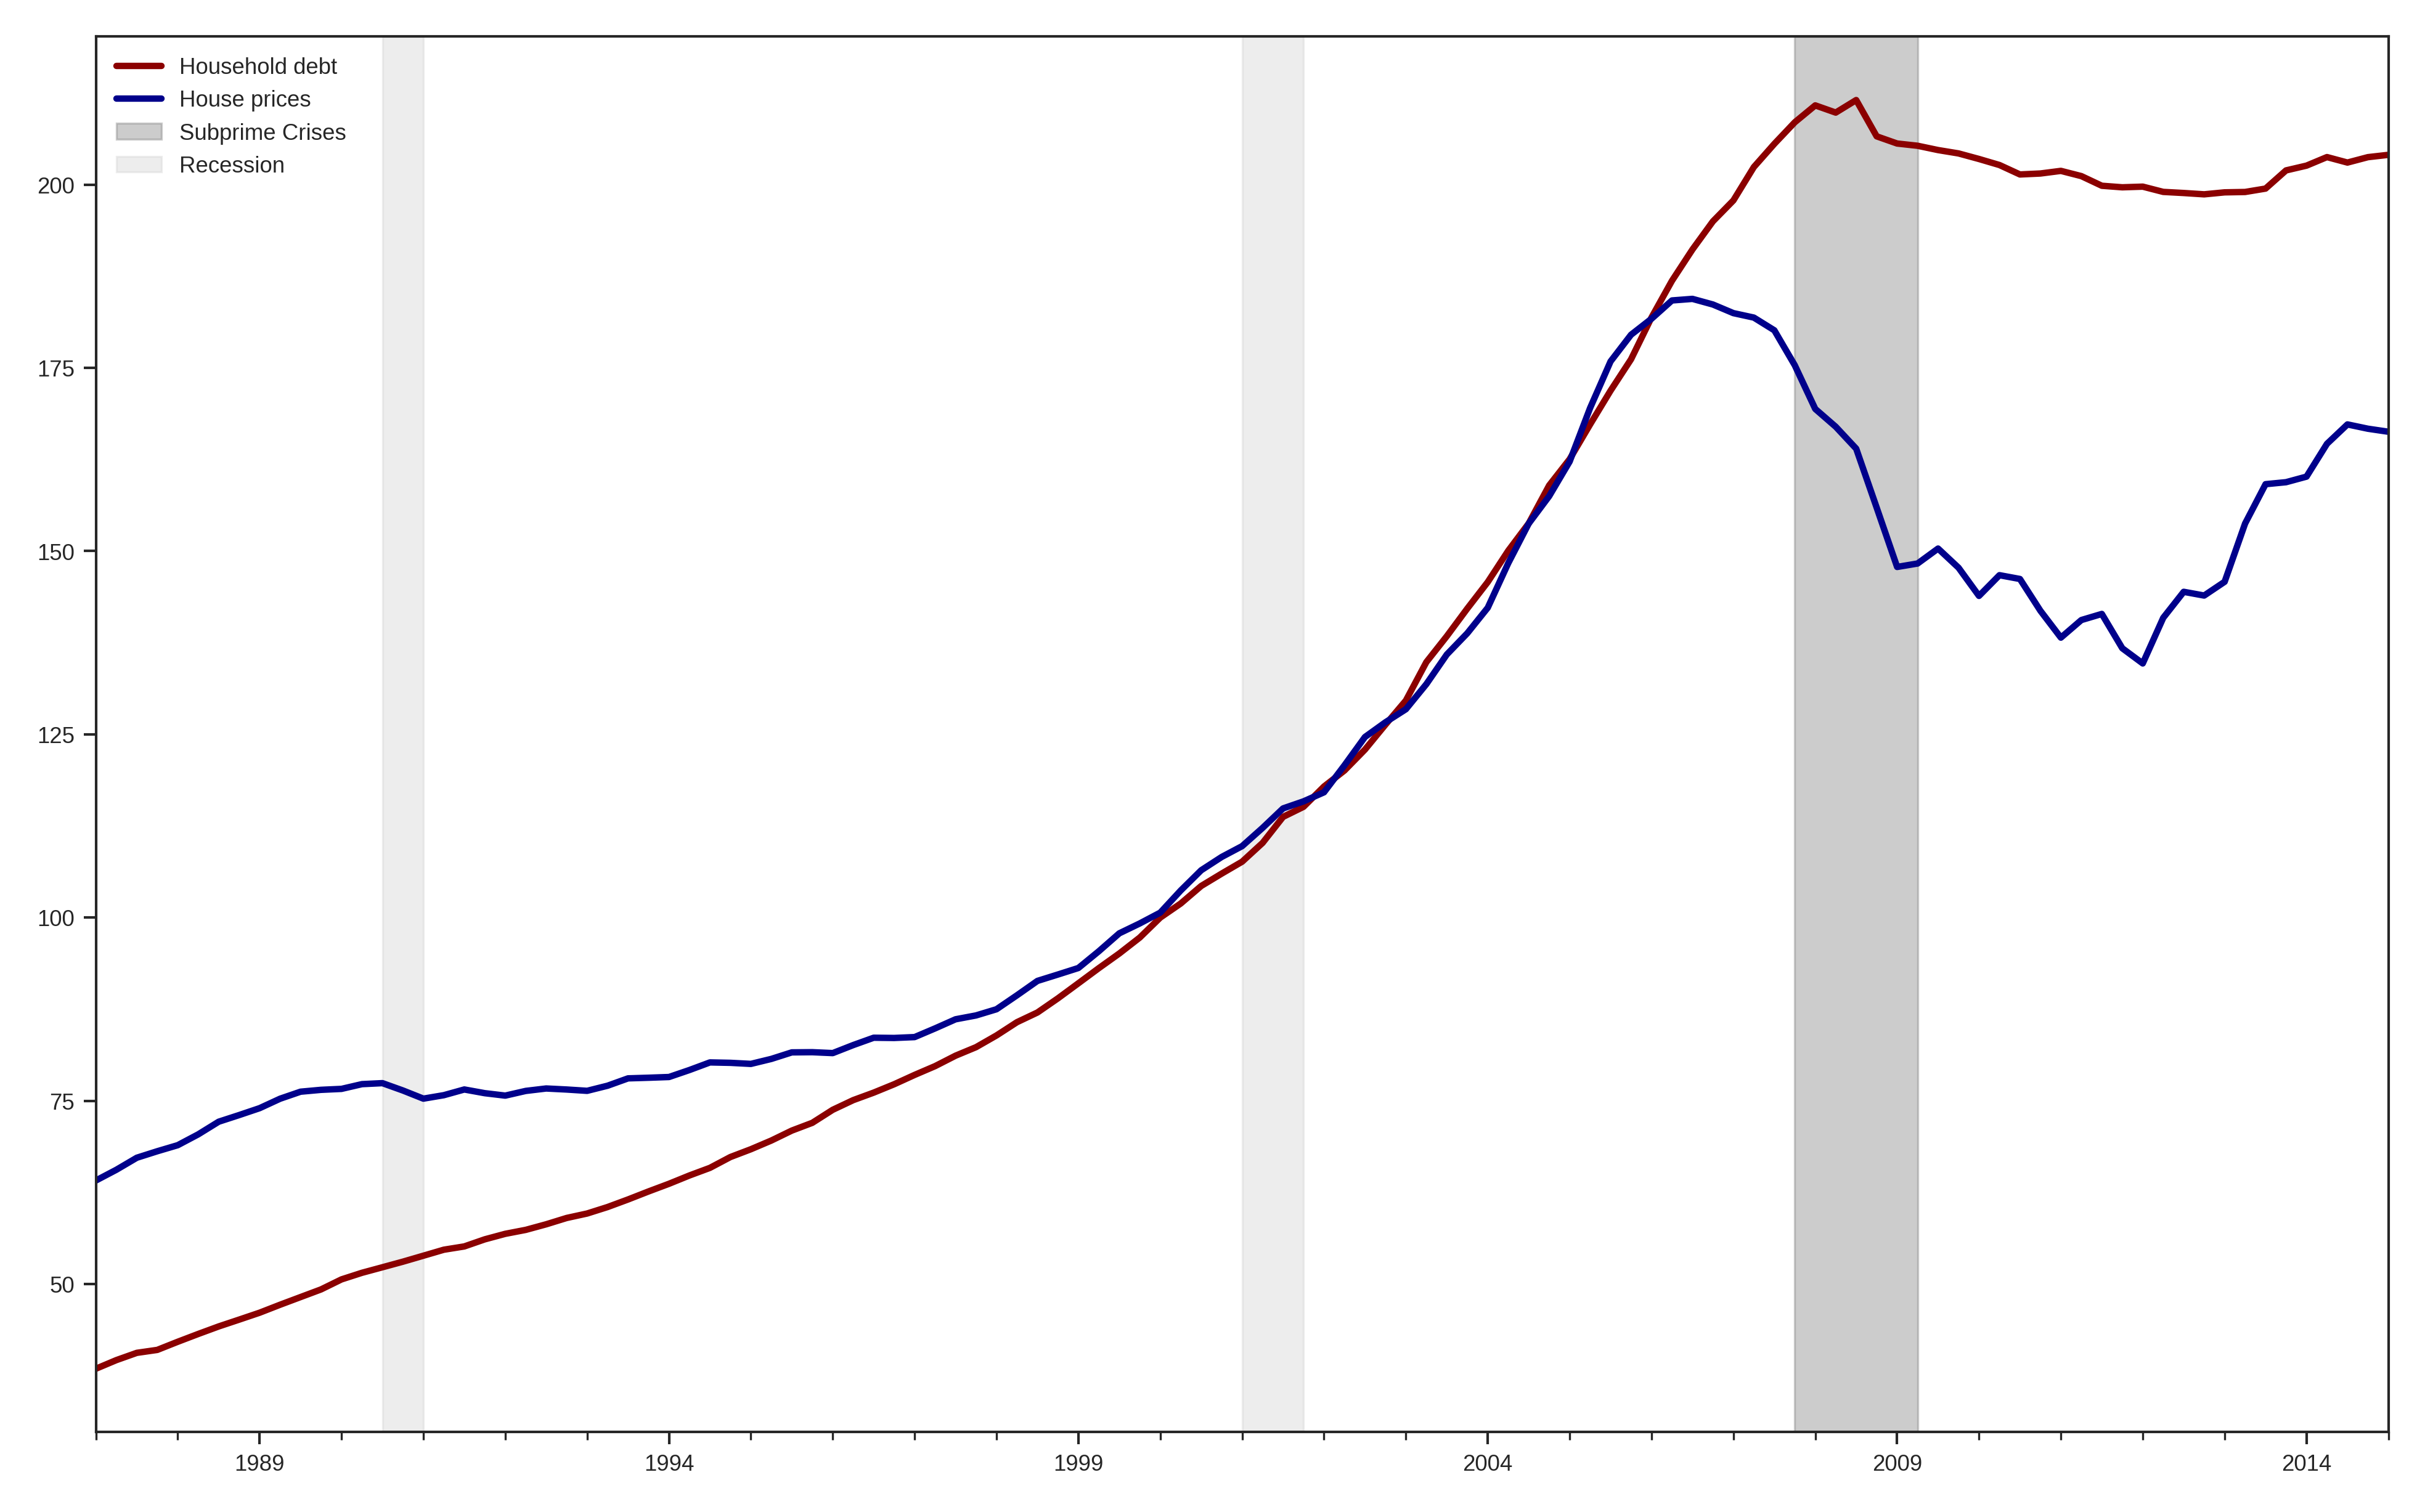
\includegraphics[width = 0.65\textwidth]{./figs/Debt_Prices.png}
    \label{fig:debt}
    \caption*{\textbf{Source:} Federal Reserve Bank of St. Louis, authors’ elaboration.}
\end{figure}



Figure \ref{fig:Durables_cycles} depicts the association between residential investment and durable goods consumption before, during and after the housing bubble.
From 1992 to 2001, both durable goods consumption and residential investment share increase as long as houses own interest rate decreases.
During the housing bubble (2001-2005), residential investment growth rate increases while houses own interest rate sharply decreases (see Figure \ref{propria_investo}).
As a result, both residential investment and durable goods consumption share have a relatively constant proportion.
On the aftermath of the housing burst (2005-2009), houses own interest rate increases and is followed by a sharp decrease in both residential investment and durable goods consumption.
Therefore, real estate inflation and durable goods consumption are connected in the U.S. and have relevant implications for the business cycle \footnote{\textcites{zezza_u.s._2008}{barba_rising_2009}, for instance, also report that credit-financed consumption was one of the main drivers of economic growth before the Great Recession.}. 

\begin{figure}[htb]
    \centering
        \caption{Residential investment share Vs. durable goods share Vs. Houses Own interest rate\\\centering Before, during and after housing bubbles\\\centering (Dots darken in  time)} 
    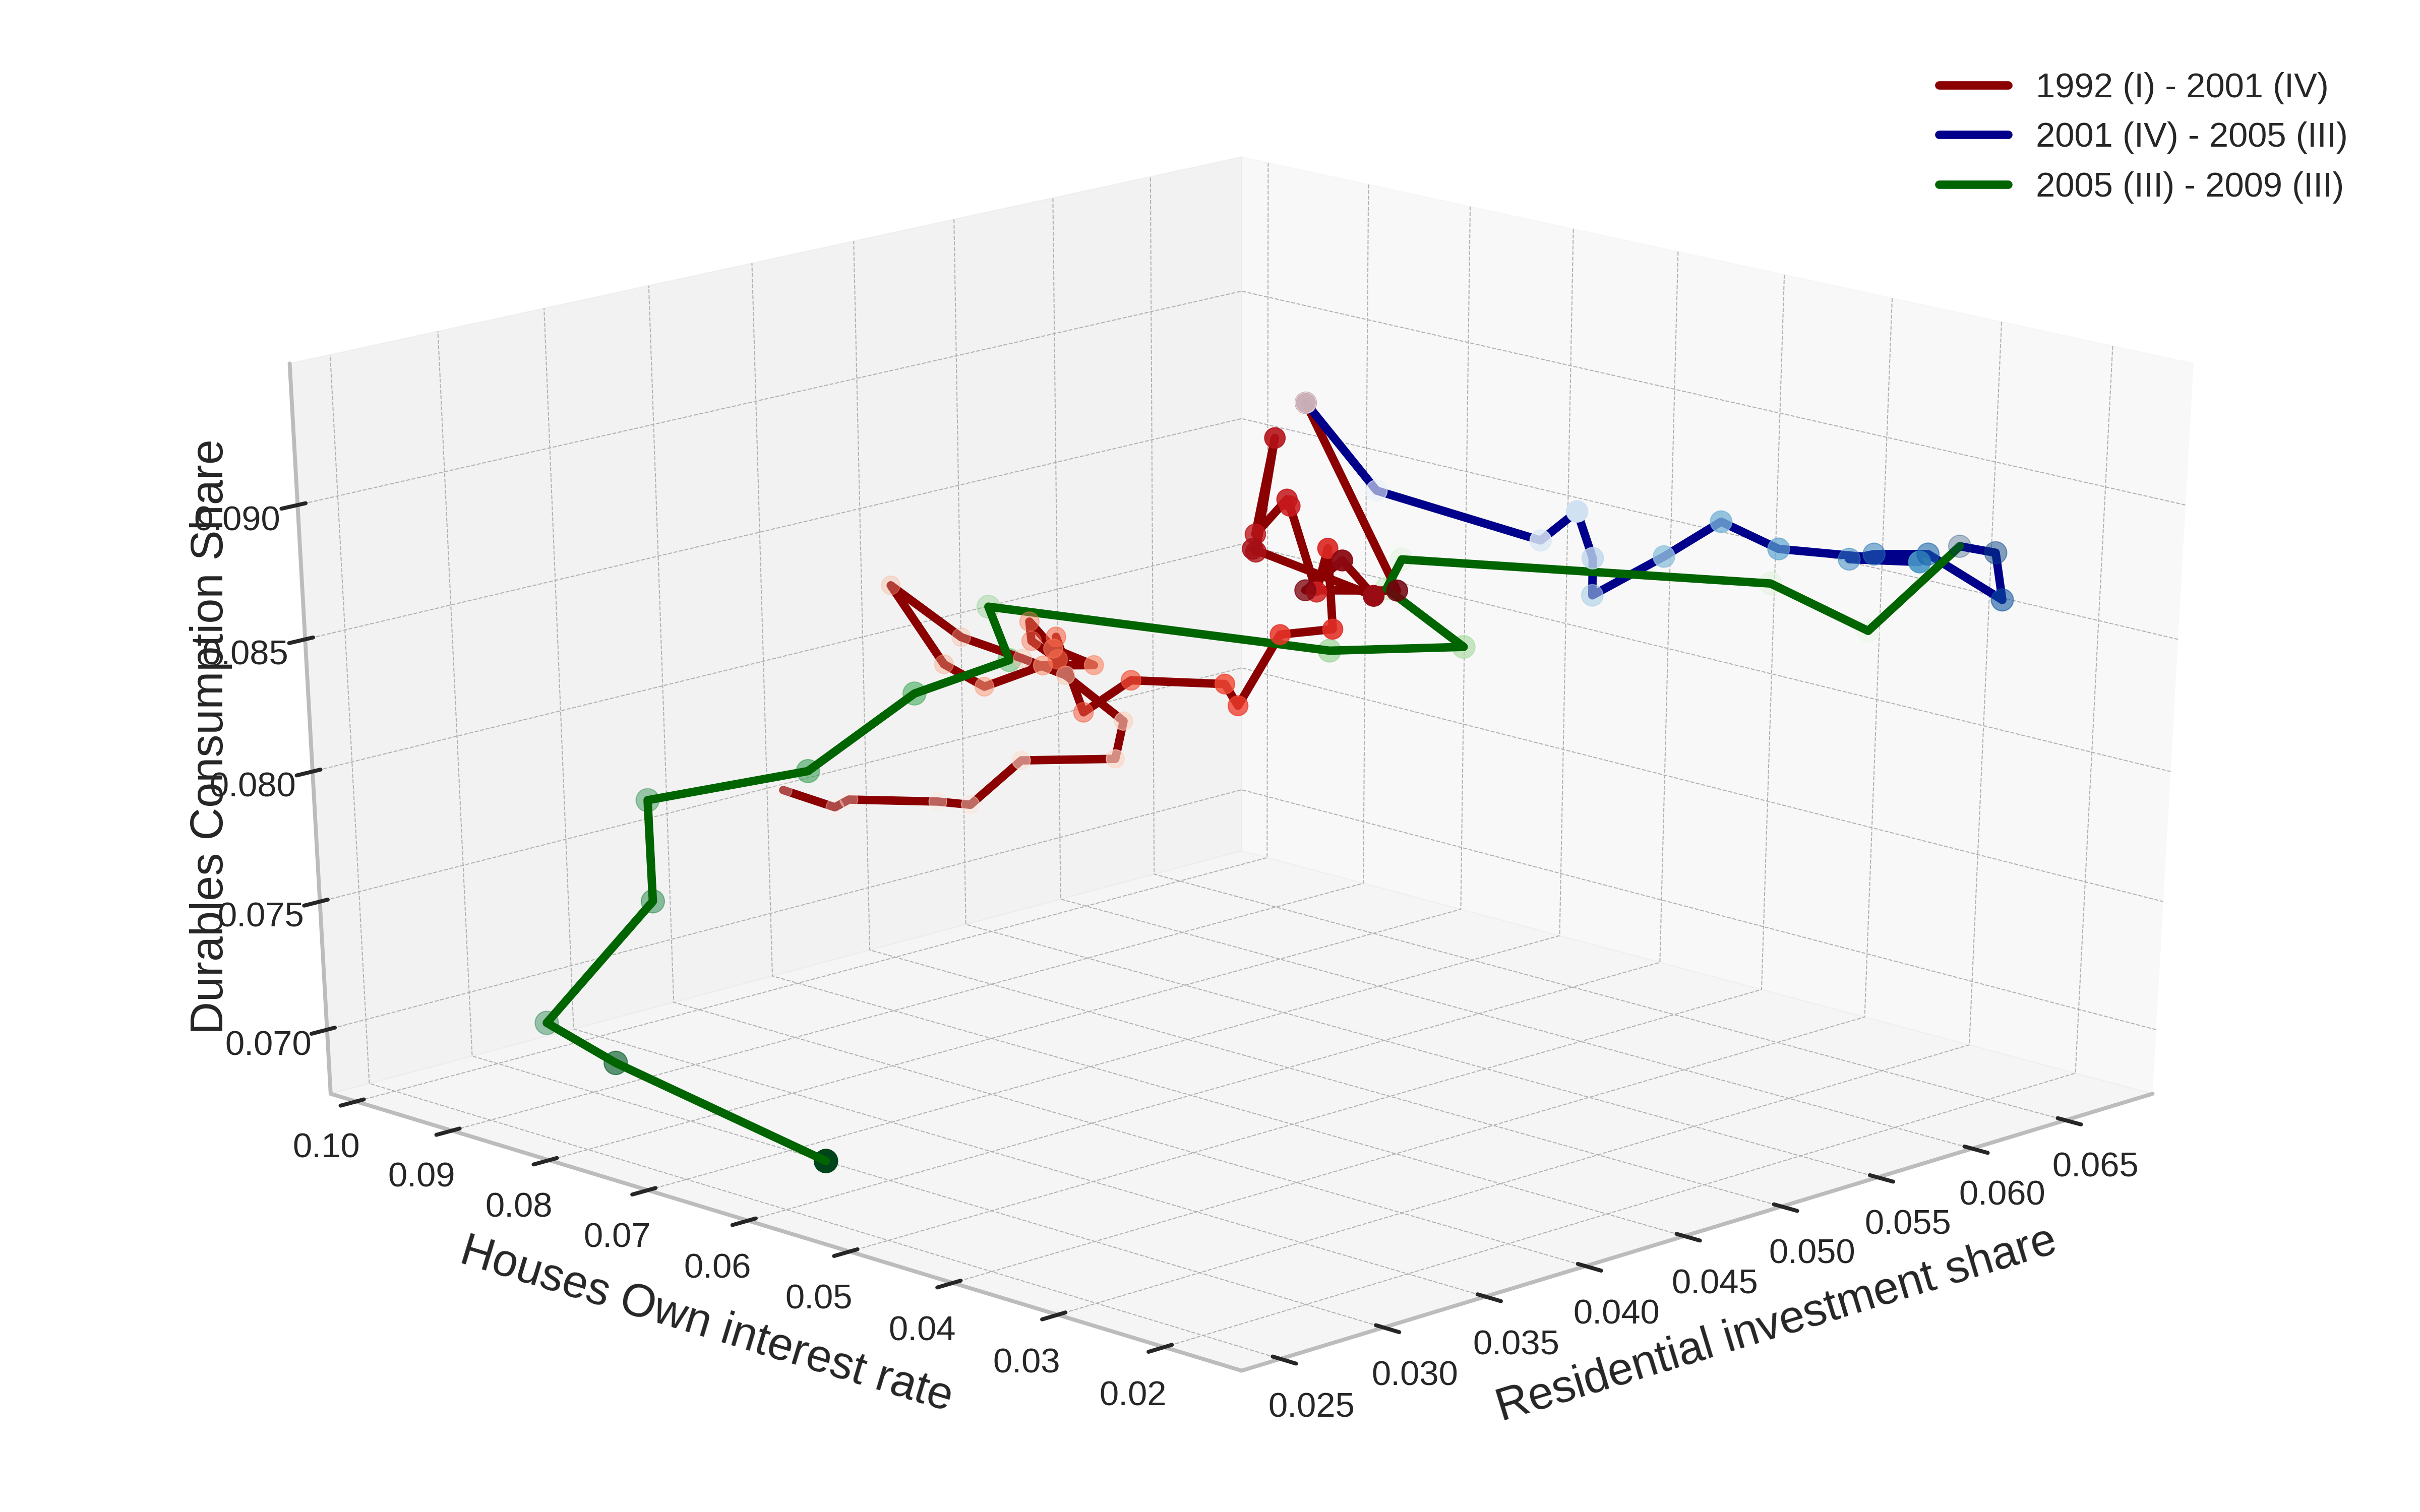
\includegraphics[width = 0.75\textwidth]{./figs/Durables_3D.png}
    \label{fig:Durables_cycles}
    \caption*{\textbf{Source:} Federal Reserve Bank of St. Louis, authors’ elaboration.}
\end{figure}



Before we move forward, it worth mentioning that the relevance of residential investment is not restricted to its growth effects nor to the U.S. 
For example, \textcite{jorda_great_2016} report that credit and financial sector growth has been led mainly by mortgages for at least 17 OECD countries\footnote{As a consequence, banking activities were redirected towards granting credit majorly to households and not to productive investment \cites{erturk_banks_2007}{kohl_more_2018}.}. 
Other studies have shown that real estate inflation describes household indebtedness and wealth distribution movements and has implications for macroeconomic stability \cites{ryoo_household_2016}{stockhammer_debt-driven_2016}{barnes_private_2016}{johnston_global_2017}{mian_household_2017}{anderson_politics_2020}{fuller_housing_2020}. 
With regard to the role of residential investment for the Great Recession, \textcite{albanesi_credit_2017} shed some light on who were the housing bubble blowers and presented higher default rates: prime rate borrowers\footnote{Contrary to the ``Old Narrative'' \cite{mian_consequences_2009},  \textcite{albanesi_credit_2017}  also report that the granting of credit and the default rate among those with the worst risk assessment remained constant throughout the housing bubble.}.
In summary, what we intended to show is that one cannot analyze the U.S. business cycle properly without considering residential investment and asset bubbles together.
On the following section, we investigate how demand-led growth theoretical literature has dealt with this topic.






\section{The absence of residential investment in demand-led growth models}
\label{sec:org19ce83d}
\label{sec:Review}

Recently, there is an effort to include SSM in Post-Keynesian strands \cite{lavoie_post-keynesian_2015}.
Some authors have explored the consequences of  different NCC autonomous expenditures through modifications in the canonical Kaleckian model \cites{allain_tackling_2015}{lavoie_convergence_2016}\footnote{This modifications in the canonical Kaleckian growth model are related to critiques regarding its non-convergence to normal utilization rate on the long-run \cites{dallery_conflicting_2011}{skott_theoretical_2012}{hein_harrodian_2012}.}.
It worth noting that both Sraffian and non-canonical Kaleckian models presents the same results on the fully-adjusted position:
(i) changes in income distribution has level effects while long-run growth rate remains unchanged;
(ii) capacity utilization smoothly converges to the normal one toward adjustment on the endogenous marginal propensity to invest;
(iii) changes in NCC autonomous expenditures growth rate has persistent effects on economy growth rate.
In this Section, we will analyze which NCC has been included and its consequences.

\textcite{allain_tackling_2015} considers tax-financed government consumption growing at an exogenous rate as NCC autonomous expenditure. 
In this precursor model, tax rate adjusts endogenously so  government budget remains balanced while growth and capacity utilization rates converge to the fully adjusted postion values.
Recently, some scholars have extended \citeauthor*{allain_tackling_2015}'s contributions related regarding other policies implications.
On the Kaleckian side, \textcite{bougrine_autonomous_2020} analyses the consequences of both fiscal and monetary expansionist policies and concludes that only the first one changes the long-run growth rate while the latter has only temporary effects.
\textcite{freitas-2020-basel-super}, on the Sraffian side, investigate the relation between autonomous expenditure growth rate, interest rate, and functional income distribution according to two Classical closures and conclude that changes on interest rate have a pure financial effect on both of them  while only one presents a (inverse) relationship with wage share\footnote{The latter Classical closure is the monetary theory of distribution proposed by \textcite{pivetti_essay_1992} in which DESCREVER TEORIA MONETÁRIA DA DISTRIBUIÇÃO.}.

\textcites{dutt_maturity_2006}{palley_inside_2010}{hein_finance-dominated_2012} present a model in which debt-financed consumption under standard neo-Kaleckian assumptions.
Thus, stability is reached only if NCC autonomous consumption grows at the same rate of capital accumulation which means that this expenditure is not really autonomous. 
\textcite{pariboni_autonomous_2015} presents an SSM alternative in which this causality is reversed so accumulation gradually converges towards debt-financed growth rate and the same results are reported by \textcite{lavoie_convergence_2016}.
\textcite{nah_long-run_2017} --- similar to \textcite{dejuan_hidden_2017} --- introduce exports as the main driver of growth. 
Despite reporting standard SSM results as well, their model has different accumulation regimes (profit-led or wage-led) depending on how real exchange rate reacts to changes in income distribution.

\textcite{brochier_supermultiplier_2018} was the first effort to introduce SSM model in a fully specified SFC framework. 
They present a non-parsimonious model in which wealth-financed consumption plays the leading role.
The results are at odds with the standard SSM model: income distribution affects fully-adjusted position growth rate.
In other words, paradoxes of thrift and costs are held despite convergence of utilization rate to the normal one.
Although causal mechanisms may not be clear --- considering the complexity of this model --- it is a  exception to what has been presented so far.
\textcite{mandarino-2020-worker-debt} also build a SSM model in a SFC framework in which debt-financed-led consumption is the NCC autonomous expenditure.
At odds with \textcite{brochier_supermultiplier_2018} and according to \textcites{pariboni_autonomous_2015}{lavoie_convergence_2016}, \textcite{mandarino-2020-worker-debt} report SSM standard results in which changes on income distribution affects growth rate only during the traverse.


Even though these works emphasize the relevance of some NCC autonomous expenditures, residential investment has been systematically neglected.
To be fair, \textcites{zezza_u.s._2008}{nikolaidi_securitisation_2015} include residential investment in a SFC growth model.
However, as a result of neo-Kaleckian non-residentialinvestment function specification, residential investment does not lead the business cycle and plays a secondary role.
From this literature review, we report an absence of residential investment-led growth models. 
Despite shedding light on some relevant relationships, \citeauthor*{teixeira_crescimento_2015}'s \citeyear{teixeira_crescimento_2015} proposition was not presented in a numerical simulation model.
The next section will present a fully specified parsimonious SSM-SFC residential investment-led model 
which its growth rate is described by the already mentioned houses own interest rate.

\section{A Sraffian supermultiplier SFC model with residential investment}
\label{sec:org319b589}
\label{sec:Model}

\subsection{General equations}
\label{sec:org1807a6b}

Our model is the most parsimonious as possible: a closed capitalist economy without government sector. Output (\(Y\)) is determined by  a fixed combination of a homogeneous labor (\(L\)) input with homogeneous fixed capacity creatin capital (\(K_f\)). 
For simplicity, we put technological progress, depreciation and goods inflation aside so investment is presented in net terms and all variables --- except for houses --- are measured in real terms.
Assuming a Leontief production function and that growth is not constrained by labor scarcity, full capacity output (\(Y_{FC}\)) is
determined by firms' capacity creating capital stock:
\begin{equation}
\label{_Leontieff}
    Y_{FC} = \min (Y_L, Y_K)
\end{equation}
\begin{equation}
\label{_YFC}
    Y_{FC} = \frac{K_{f_{-1}}}{v}
\end{equation}
\begin{equation}
\label{_u}
    u = \frac{Y}{Y_{FC}}
\end{equation}
where \(Y_L\) and \(Y_K\) stands for full employment and full capacity output respectively, \(v\) is exogenous capital-output ratio and \(u\) is utilization rate.

We further assume a ``Kaleckian'' economic structure composed by both workers (denoted by \(w\)) and capitalists (denoted by \(k\)) households.
In accordance with \textcite{albanesi_credit_2017}, we consider that only the latter invest in real estate and are not credit constrained.
Thus, demand-determined output level (\(Y\))  is the sum of workers and capitalists consumption (\(C_w\) and \(C_k\) respectively) and both households and firms investment (\(I_h\) and \(I_f\) respectively) and only the latter creates capacity to the business sector of the economy:
\begin{equation}
\label{_Ct}
    C = C_w + C_k
\end{equation}
\begin{equation}
\label{_It}
    I_t = I_f + I_h
\end{equation}
\begin{equation}
\label{_Y}
    Y = \overbrace{[C_w + \underbrace{C_k + I_h}_{\text{Capitalists}}]}^{\text{Households}} + \overbrace{[I_f]}^{\text{Firms}}
\end{equation}

In other words, from institutional sectors perspective, household expenditures have two components (consumption and residential investment) and firms just one (non-residential investment). 
Only non-residential investment creates productive capacity. 
So, the novelty of this model is the inclusion of a second investment component all made by household sector and held by capitalists households for simplicity. 
Therefore, this economy produces two types of real assets: firms productive capital (\(K_f\)) and households housing (\(K_h\)):
\begin{equation}
    \label{_K}
    K = K_f + K_h
\end{equation}

Denoting the houses share in total real assets as \(k\), we can rewrite equation \ref{_K} as:
\begin{equation}
\label{_k}
    k = \frac{K_h}{K}
\end{equation}
$$
K = (1-k)\cdot K + k\cdot K
$$

Following both Sraffian and Kaleckian strands, we assume exogenous functional income distribution which allows us to define total wages (\(W\), Eq. \ref{_W}) as a function of wage-share (\(\omega\)):

\begin{equation}
\label{_W}
    W = \omega\cdot Y
\end{equation}

Table \ref{Matriz_Estoques} presents the balance sheet matrix for all institutional sectors. 
Capitalists households hold financial wealth as bank deposits (\(M\)) and residential investment is financed by mortgages (\(MO\)).
Capitalists' total net wealth (\(NW_{k}\)) is the sum of their net financial wealth (\(V_{k}\)) and real assets (\textit{i.e.} housing, \(K_h\)). 
Furthermore, capitalist consumption (\(C_k\)) is fully autonomous and financed by loans (\(L_{k}\)) while workers consumption (\(C_w\)) is fully induced by their wages.
As usual, we assume that workers expend what they earn while capitalists earn what they expend, so workers financial and real wealth are both null.
Firms finance their investment primarily by undistributed profits (\(FU\)) and the residual by bank loans (\(L_f\)) --- thus they do not hold deposits. 
Banks create credit \textit{ex nihilo} and then collect the deposits, paying the same interest rate that they charge.

\begin{table}[H]
\centering
\caption{Balance Sheet matrix}
\label{Matriz_Estoques}
\begin{tabular}{lccccc}
\hline
\hline
                          & Workers & Capitalists      & Firms        & Banks  &    $\sum$ \\ \hline

Deposits & & $+M$ & & $-M$ & 0\\
Loans& &$-L_{k}$ &$-L_f$& $+L$ & 0\\
Mortages & &$-MO$&  & $+MO$ & 0\\\hline
$\sum$ Net Financial Wealth &--- &$V_{k}$&$V_f$&$V_b$& $0$\\\hline
Capital & & &$+K_f$&  & $+K_f$\\
Houses & &$+K_{hd}$& &   & $+K_h$\\\hline
$\sum$ Net Wealth &---&$NW_{k}$&$NW_f$&$NW_b$& $+K$\\
\hline
\hline
\end{tabular}%
\caption*{\textbf{Source:} Authors' Elaboration}
\end{table}

Table  \ref{Matriz_Fluxos} presents both transactions flows and the flow of funds matrix. 
This table shows all economic relations between institutional sectors ensuring that there is no  ``black holes''
so all financial and real transaction are explicit \cite{macedo_e_silva_peering_2011}.

\begin{table}[H]
\centering
\caption{Transactions flow matrix and flow of funds
}
\label{Matriz_Fluxos}
\resizebox{\textwidth}{!}{%
\begin{tabular}{lccccccc}
\hline
\hline
& Workers
& \multicolumn{2}{c}{Capitalists}
& \multicolumn{2}{c}{Firms}                        
& Banks       & Total    \\ \cline{3-4}\cline{5-6}
& &
Current & Capital & 
Current & Capital     & 
&       $\sum$ \\ 
Consumption                       &$-Cw$&$-C_k$& & $+C$& & & 0\\
Non-residential Investment                   & & & &$+I_f$&$-I_f$ & & 0\\
Residential Investment       &  & &$-I_h$&$+I_h$& & & 0\\
\textbf{{[}Output{]}}   & & & &{[}$Y${]}& & & {[}$Y${]}\\
Wages                        &$+W$&& &$-W$& & & 0\\
Profits                      & &$+FD$& &$-FT$&$+FU$& & 0\\
Deposits interest rate         & &$+r_m\cdot M_{-1}$& && &$-r_m\cdot M_{-1}$& 0\\
Loans interest rate         & &$-r_l\cdot L_{k_{-1}}$& &$-r_l\cdot L_{f_{-1}}$& &$+r_l\cdot L_{-1}$& 0\\

Mortages interest rates         & &$-r_{mo}\cdot MO_{-1}$& && &$+r_{mo}\cdot MO_{-1}$& 0\\\hline
\textbf{Subtotal}           &---&$+S_h$&$-I_h$& &$+NFW_f$&$+NFW_b$& 0\\\hline
Change in deposits     & &$-\Delta M$& & & &$+\Delta M$& 0\\
Change in mortgages     & & &$+ \Delta MO$& & &$-\Delta MO$& 0\\
Change in loans     & &$+\Delta L_{k}$&&$+\Delta L_f$& &$-\Delta L$& 0\\
\textbf{Total} & & 0 & 0 & 0  & 0  & 0  & 0\\
\hline
\hline
\end{tabular}%
}
\caption*{\textbf{Source:} Authors' Elaboration}
\end{table}


\subsection{Firms}
\label{sec:orga726a91}

In order to produce, firms purchase capital goods (\(-I_f\) in capital account) and hire workers, whom total remuneration is the economy wage bill. 
Their total profits (\(FT\)) are a residual between sales (\(Y\)) and total wages (\(W\)). 
Firms retain part (\(\gamma_F\)) of profits net of interest payments (\(FU\)) --- to reinvest --- and distribute the rest to capitalists (\(FD\)):

\begin{equation}
\label{_FT}
    FT = Y - W = FD + FU
\end{equation}
\begin{equation}
    FU = \gamma_F\cdot (FT - r_l\cdot L_{f_{-1}})
\end{equation}
\begin{equation}
    FD = (1-\gamma_F)\cdot (FT - r_l\cdot L_{f_{-1}})
\end{equation}

Firms (non-residential) investment is fully induced by the level of effective demand \cite{freitas_growth_2015}, and its growth rate changes accordingly to the capital stock adjustment principle. 
This implies that firms react to the discrepancies between actual and normal utilization rates (\(u_N\)). 
As mentioned above, only firms investment creates productive capital stock.

\begin{equation}
\label{_If}
    I_f = h\cdot Y
\end{equation}
\begin{equation}
\label{_h}
    \Delta h = h_{t-1}\cdot \gamma_u\cdot (u - u_N)
\end{equation}
\begin{equation}
    \Delta K_f = I_f
\end{equation}
where \(h\) is (endogenous) marginal propensity to invest and \(\gamma_u\) must be sufficiently small in order to the adjustment be gradual\footnote{The size of this parameter guards a fundamental relation to the stability of the model, as shown by \textcite{freitas_growth_2015}.}.

Firms finance part of investment that exceeds undistributed profits by bank loans, paying an interest rate on it (\(r_l\)) charged by the banks. 
We assume an elastic supply of credit for investment. 
Moreover, tables \ref{Matriz_Estoques} and \ref{Matriz_Fluxos} show firms net wealth (\(NW_f\)) and net financial balance (\(NFW_f\)) explicitly:

\begin{equation}
\label{_Lf}
    \Delta L_f = I_f - FU
\end{equation}
$$
r_g = \frac{\pi\cdot u}{v}
$$
$$
r_n = r_g - r_l\cdot\frac{L_{f_{-1}}}{K_f}
$$
\begin{equation}
    NFW_f = FU - I_f
\end{equation}
\begin{equation}
    NW_f = K_f - L_f
\end{equation}
where \(r_g\) and \(r_n\) denotes gross and net profit rate respectively.


\subsection{Banks}
\label{sec:org05bcf77}

As in most part of SFC literature, banks do not have an active role in our model.
They create money as credit is demanded and just after they collect deposits \cite{le_bourva_money_1992}. 
Firms finance part of their investment with credit (\(L_f\)) and capitalists households finance all their residential investment by mortgages (\(MO\)) and consumption by loans (\(L_{k}\)), as already mentioned. 
Each operation has its own interest rate defined by a spread (\(\sigma_l\) and \(\sigma_{mo}\)) over deposits interest rate (\(r_m\)) exogenously determined by banks.
For simplicity, we assume null bank spreads so interest rate on mortgages and on loans
are the same as on deposits.
Banks net balances (\(NFW_b\)) are defined by interests received net of interests payments. 
As those interests are the same, banks net wealth is necessarily zero (see table \ref{Matriz_Estoques}) and deposits are residuum:

\begin{equation}
L = L_f + L_{k}
\end{equation}
\begin{equation}
    r_l = (1+\sigma_l)\cdot r_m
\end{equation}
\begin{equation}
    r_{mo} = (1+\sigma_{mo})\cdot r_m
\end{equation}
\begin{equation}
    r_m = \overline r_m
\end{equation}
\begin{equation}
    NFW_b = r_{mo}\cdot MO_{-1} + r_l\cdot L_{-1} - r_m\cdot M_{-1}
\end{equation}
$$
NFW_b = \Delta MO + \Delta L - \Delta M
$$
\begin{equation}
    NW_b = V_b \equiv 0
\end{equation}
\begin{equation}
\label{_M}
    \Delta M = \Delta L + \Delta MO
\end{equation}

\subsection{Households}
\label{sec:org2b4ee30}

\subsubsection*{Workers}
\label{sec:org31b0a7c}
As mentioned before, we assume that workers expend (\(C_w\)) what they earn (\(W\)). 
For simplicity, we consider that wages are the only source of income workers' disposable income (\(YD_{w}\)) and do not have access to consumption loans, so worker' saving (\(S_{hw}\)) are null.
Therefore, accordingly to our hypothesis, workers' do not hold both net financial and total wealth.

\begin{equation}
C_w = W
\end{equation}
\begin{equation}
YD_w = W
\end{equation}
\begin{equation}
S_{w} = YD_w - C_w
\end{equation}
$$
S_{w} = 0
$$
\begin{equation}
NFW_{w} = S_{w} = 0
\end{equation}
\begin{equation}
V_{w} = 0
\end{equation}

\subsubsection*{Capitalists}
\label{sec:orge25bccc}
This is the most complex institutional sector of our model. 
We assume consumption (\(C_k\)) is fully-autonomous and financed by loans (\(L_{k}\)). 
Disposable income (\(YD_k\)) is the sum of distributed profits and received interests on deposits, net of interests payments
on both mortgages and loans.
Capitalists savings (\(S_{k}\)) are disposable income net of consumption.
At odds with SFC literature, savings are not equal to net balance (\(NFW_{k}\)) since we have included residential investment.

\begin{equation}
\Delta L_{k} = C_k
\end{equation}
\begin{equation}
    \label{EqYD}
    YD_k = FD + \overline r_m\cdot M_{-1} - r_{mo}\cdot MO_{-1} - r_{l}\cdot L_{k_{-1}}
\end{equation}
\begin{equation}
    \label{EqSh}
    S_{k} = YD_k - C_k
\end{equation}
\begin{equation}
\label{NFWh}
    NFW_{k} = S_{k} - I_h
\end{equation}

In order to fulfill our goals, we employ \citeauthor*{freitas_baseline_2019}'s \citeyear{freitas_baseline_2019} procedure in which NCC autonomous expenditure (\(Z\)) composition (\(R\)) remains unchanged so we express capitalists and total consumption as follows:

\begin{equation}
    \label{EqMO}
    \Delta MO = I_h
\end{equation}
\begin{equation}
\label{_Z}
Z = C_k + I_h
\end{equation}
$$
\frac{C_k}{Z} + \frac{I_h}{Z} = R + (1-R)
$$
\begin{equation}
\label{_Ck}
    C_k = R\cdot Z
\end{equation}
\begin{equation}
\label{ConsumoTotal}
C = C_w + C_k
\end{equation}
$$
C = C_w + R\cdot Z
$$
which allows us to rewrite both NCC and autonomous consumption in terms of residential investment (Eq. \ref{Z_Ih}):
\begin{equation}
\label{Z_Ih}
Z = \frac{I_h}{(1-R)}
\end{equation}

\begin{equation}
\label{C_kZ}
C\textsubscript{k} = I\_h\(\cdot\) \frac{R}{(1-R)}
\end{equation}


As households are the only institutional sector investing in real estate, its supply (\(I_{hs}\)) and demand (\(I_h\)) are equal and the same applies to its stock.
\begin{equation}
    I_{hs} = I_h
\end{equation}
\begin{equation}
    K_{hs} = K_{hd}
\end{equation}
\begin{equation}
    \Delta K_{hs} = \Delta K_{hd} = I_{hs} = I_h
\end{equation}
where \(S\) and \(D\) denote supply and demand respectively. 
Accordingly to our hypothesis, nominal (\(V_{k}\)) and real net wealth (\(V_{kr}\)) are distinguished only by the inclusion of real estate price (\(p_h\)) and are defined as follows:
\begin{equation}
V_{k} = K_{hd}\cdot p_h + M - L_{k} - MO
\end{equation}
\begin{equation}
V_{kr} = K_{hd} + M - L_{k} - MO
\end{equation}

Finally, we present residential investment growth rate (\(g_{I_h}\)) as determined by houses own interest rate (\(own\), equation \ref{_own}) as introduced by \textcite{teixeira_crescimento_2015} and discussed in section \ref{sec:empirical}.

\begin{equation}
    I_h = (1 + g_{I_h})\cdot Ih_{-1}
\end{equation}
\begin{equation}
\label{g_Z_own}
g_{I_h} = \phi_0 - \phi_1\cdot own
\end{equation}

\begin{equation}
\label{_own}
own = \left(\frac{1+r_{mo}}{1+\pi}\right) -1
\end{equation}
$$
\pi = \frac{\Delta p_h}{p_{h_{t-1}}}
$$
where \(\pi\) stands for real estate inflation, \(\phi_0\) represents long-term determinants (\emph{e.g.} demographic factors, housing and credit policies, etc.) while \(\phi_1\) captures the demand for real estate arising from expectations of capital gains resulting from speculation with the existing dwellings stock. 
Finally, replacing Equation \ref{Z_Ih} in \ref{_Ck}, we can describe NCC autonomous expenditure growth rate as follows:
\begin{equation}
\label{g_Z}
g\textsubscript{C\textsubscript{k}} = g\textsubscript{Z} = g\textsubscript{I\textsubscript{h}} = \(\phi\)\textsubscript{0} - \(\phi\)\textsubscript{1}\(\cdot\) own
\end{equation}

In this section, we presented our fully-specified parsimonious model to represent the U.S economy (1992-2019). It worth mentioning that, although simplified, our hypotheses are supported by recent empirical evidence \cites{albanesi_credit_2017}. Following \textcites{teixeira_crescimento_2015}{petrini_demanda_2019}, we specify a econometrically significant residential investment growth rate function which allows us to include housing bubbles in the SMM model. On the next Section, we present the short-run and fully-adjusted position dynamics in order to show the particularities of a model with two types of capital stock in the presence of asset bubble.




\section{Short and long-run equilibria}
\label{sec:org34bdbb7}
\label{sec:runs}

In this Section, we show the implications residential investment inclusion into a SSM-SFC model. First, we present the short-run dynamics and then move to the fully-adjusted position (denoted by \(\star\)).

\subsection{Short-run good market equilibrium}
\label{sec:org057dc09}
\label{short}

In our no-government closed economic system, real output (equation \ref{_Y}) is the sum of household consumption (equation \ref{ConsumoTotal}) and both types of investment (equation \ref{_It}). 
If we replace equations \ref{_W} and  \ref{_If} into \ref{_Y} and considering equation \ref{_Z} we get the short-run GDP level:



\begin{equation}
\label{AnaliticaNivel}
36 - aeb49019-e5c1-4a0b-9b16-8aee5c9c5ee1 <output> <interrupt>
\end{equation}

Next, dividing equation \ref{AnaliticaNivel} by \ref{_YFC} and presenting firm's capital stock in terms of \(k\), we get the short-run equilibrium utilization rate (Eq \ref{short_u})


\begin{equation}
\label{short_u}
37 - 0dfc2999-c0e7-45aa-b1fc-1c07f131e3f8 <output> <interrupt>
\end{equation}

So, rearranging Equation \ref{short_u} in terms of houses,
$$
u_{t} = Y\frac{v}{K_{HD}}\cdot \frac{k_{t}}{1-k_{t}}
$$

\begin{equation}
\label{u_houses}
u_{t} = \frac{1}{1-R}\cdot \frac{g_Z\cdot v}{1 - \omega - h_{t}}\cdot \frac{k_{t}}{1-k_{t}}
\end{equation}
which allows us to present houses share on total capital stock of the economy
\begin{equation}
\label{k_short}
k = 1 - \frac{v\cdot g_Z}{(1 - \omega)\cdot u_{t}}
\end{equation}


Finally, we present short-run growth rate following \textcite{freitas_growth_2015}:

\begin{equation}
\label{g_short}
g_t = g_{Z} + \frac{\Delta h}{1 - \omega - h_{t}}
\end{equation}
On the following subsection, analyze the fully-adjusted positions values and steady state stock/flow ratios.


\textbf{Nota:} Não organizei bem o texto desta seção. Não tenho certeza se essa é a melhor ordem de apresentação das equações, mas acredito que isso seja rápido de corrigir.

\subsection{Fully-adjusted position}
\label{sec:orgba7ef48}
\label{long}


As mentioned before, endogenous firms’ marginal propensity to invest reacts to discrepancies between the utilization rate and the normal one.  During the adjustment process (\(u\to u_N\)), GDP growth rate moves towards NCC autonomous expenditure growth rate (in this case, residential investment and capitalist consumption):

$$
u \to u^{\star}  = u_N \Leftrightarrow g \to g^{\star} = g_Z
$$
and (endogenous) fully-adjusted position marginal propensity to invest will be:


\begin{equation}
\label{h_long}
h^{\star} = g^{\star}\cdot \frac{v}{u^{\star}}
\end{equation}

Next, we move towards the analysis of the particularities of our model:  one of the NCC autonomousexpenditures also contributes to capital stock accumulation.  
Replacing Equation \ref{h_long} in \ref{k_short}, we obtain fully-adjusted position of the ratio between housesand total capital stock (denoted by \(k^\star\)). It worth noting that the second term of RHS of equation \ref{k_long} is equal to the so-called ``fraction'' (\(f\)) introduced by \textcite{serrano_long_1995}:

\begin{equation}
\label{k_long}
k^{\star} = 1 - \frac{h^{\star}}{1-\omega}
\end{equation}

$$
k^{\star} = 1 - f \hspace{3cm} f = 1 - k^{\star}
$$


Before moving on to the numerical simulations, we present some steady state stock/flow ratios in order to shed some light in the dynamic process of the model. Dividing Equation \ref{_Lf} by firms' lagged capital stock and making some algebraic manipulation, we obtain steady state loans' ratio to capital stock (\(\ell^{\star}\), Equation \ref{firm_ratio}):

$$
\Delta \left(\frac{L_{f}}{K_{f}}\right) = \frac{I_{f} - FU}{K_{f}} - \ell^{\star}_{f}\cdot g^{\star}  = 0
$$

38 - 34923489-3bde-45b4-8844-7d438c018b2b <output> <interrupt>

Next, we present capitalists' loans to houses stock ratio and  rewrite capitalists autonomous expenditure in terms of residential investment (Equation \ref{C_kZ})

$$
\Delta \left(\frac{L_k}{K_{HD}}\right) = \frac{C_k}{K_{HD}} - \ell^{\star}_{k}\cdot g^{\star} = 0
$$
39 - 5f5ffe43-24f8-42a4-af53-4272f7d1e6d5 <output> <interrupt>

The same procedure can be applied to find mortgage to house stock ratio (\(mo^{\star}\), Equation \ref{mortgage_ratio}):
$$
\Delta \left(\frac{MO}{K_{HD}}\right) = \frac{\Delta MO}{K_{HD}} - mo^{\star}\cdot g^{\star} = 0
$$
40 - ca9002b3-ab2d-45b1-b8fb-4c6012fb9cac <output> <interrupt>

Finaly, we can express deposits share on total capital stock (\(m^{\star}\)) in terms of previous stock/flow ratios:

$$
\frac{M}{K} = \frac{MO + L_k + L_f}{K}
$$
$$
\frac{M}{K} = \frac{MO}{K_{HD}}\cdot \frac{K_{HD}}{K} +  \frac{L_k}{K_{HD}}\cdot \frac{K_{HD}}{K} +  \frac{L_f}{K_{f}}\cdot \frac{K_{f}}{K}
$$

\begin{equation}
\label{M_long_intermediate}
m\textsuperscript{\(\star\)} = mo\textsuperscript{\(\star\)}\(\cdot\) k\textsuperscript{\(\star\)} + \(\ell\)\textsuperscript{\(\star\)}\textsubscript{k}\(\cdot\) k\textsuperscript{\(\star\)} + \(\ell\)\textsuperscript{\(\star\)}\textsubscript{f}\(\cdot\) (1-k\textsuperscript{\(\star\)})
\end{equation}
Thus, replacing Equations \ref{h_long}, \ref{k_long}, \ref{firm_ratio}, \ref{capitalist_ratio} and \ref{mortgage_ratio} in to \ref{M_long_intermediate}, we obtain steady state deposits to total capital stock ratio (Equation \ref{deposits_rhs}\footnote{Since banks deposits are a residuum, we could express Equation \ref{deposits_rhs} in terms of Equations \ref{EqYD}, \ref{EqSh} and --- assuming null spread on mortgage and on loans interest rate --- we can rewrite net interest rate income as follows 
$$rm\cdot (M - L_k - MO) = rm\cdot (L_f)$$
So, we achieve the same result of Equation \ref{deposits_rhs} as expected.}):


41 - f69b211b-c651-4b65-ae63-a266a5e381c9 <output> <interrupt>

Before moving on to the numerical simulations, it worth noting that --- besides its counterintuitivity --- the decrease of \(k^{\star}\) as a result of the increase of residential investment growth rate (reported in equations \ref{partial_phi0} and \ref{partial_pi} in Appendix \ref{append:Solution}) is in line with the SSM.
Since firms' investment grows (temporally) at a higher pace than NCC autonomous expenditures, it has only a level effect on capital stock.
As usual, changes in income distribution affects GDP temporally.
However, it has permanent effects over capital stock composition as a result of this level effect reported before (equation \ref{partial_omega}).


\section{Numerical Simulations}
\label{sec:orgb315581}
\label{sec:Experiments}


In this Section, we present the results of the following experiments\footnote{Simulation scripts are available under request. It worth noting that our experiments are simulated using \emph{pysolve3} package available at \url{https://github.com/gpetrini/pysolve3}. Implementation and improvement requests are welcome.}: 
    (i) wage-share decrease;
    (ii) real estate inflation and;
    (iii) deposits interest rate increase.
In order to evaluate if our model is able to reproduce some stylized facts, we introduce U.S. houses own interest rate observed data (from 1992 to 2019) into our numerical simulation.
Before we move foward, it worth mentioning that we use \citeauthor*{fazzari-2020-deman-led}'s  \citeyear{fazzari-2020-deman-led} parameter values callibrated for the U.S. economy for a similar time range (from 1980 to 2016).
Since we use a SFC framework, first experiment assess if income distribution affects fully-adjusted position growth rates temporal --- as in \textcite{mandarino-2020-worker-debt} --- or persistently ---  as in \textcite{brochier_supermultiplier_2018}.
Real estate increase experiment is motivated by recent US experience (from 1992 to 2019) as discussed in Section \ref{sec:empirical} while the last one aims to evaluate indebtedness stability.
Table \ref{tab:param} in Appendix \ref{append:Data} presents the parameters of simulation and Table \ref{ResumoChoques} compare each result to baseline.

\subsection{Wage-share decrease}
\label{sec:org6f1aa8d}
\label{sec:Exp1}

A wage-share decrease has a temporary negative impact both in GDP level and capacity utilization rate due to changes on the supermultiplier (see Figure \ref{fig:results_1}).
As a consequence of this negative level effect, both accumulation growth rate and marginal propensity to invest decline while NCC autonomous expenditures share on GDP increases.
Since NCC autonomous expenditure growth rate remains unchanged, this negative level effect is followed by a increase in non-residential investment growth rate because firms react to the discrepancies between actual and normal utilization rates.
In summary, we report standards SSM model results:
    (i) marginal propensity to invest decrease is temporally and returns to baseline level;
    (ii) utilization rate moves towards normal one;
    (iii) supermultiplier decreases and autonomous expenditure share increases due to GDP decline and; 
    (iv) since autonomous expenditure growth rate does not change, distribution effects are temporally.

Despite temporary effects in growth rate, wage-share decrease has a permanent effect in house share on total capital stock (see Equation \ref{_k_star} and Figure \ref{fig:results_2}).
As a consequence of the initially lower accumulation rate, total capital stock (firms' and households') also grows at a temporarily lower rate.
However, since residencial investment growth rate remains unchanged, its share on total capital stock increases.
Another persistent effect is the higher capitalists' indebtedness despite the profit-share increase.
This result stems from the negative level effect on profits as a consequence of the negative effect on GDP and subsequent decrease in capitalists' disposable income.
In other words, we report a paradox in capitalists attempt to increase their profit share which results a negative effect both on net profits and capitalists' disposable income.

Finally, we also report a persistent effect on firms' balance sheet due to wage-share decrease.
The negative level effect on GDP implies an already mentioned temporally decrease in marginal propensity to invest.
As a consequence of the initially lower accumulation ratio and higher profit share, firms require less external funding --- as profits distribution policy remains the same  --- so its indebtedness decreases.
Therefore, gross and net profit rate remains persistently close to each other (see Figure \ref{fig:results_2}).

\textbf{Nota:} Farei referência às equações stock/flow quando terminar esta seção

\subsection{Real estate inflation}
\label{sec:orgf9a3799}
\label{sec:Exp2}


Real estate inflation implies a higher residential investment growth due to houses own interest rate decrease.
As a result, both GDP growth rate and capacity utilization rate increase as well.
Since firms react to discrepancies between actual and normal utilization rates, non-residential investment growth rate 
is temporally higher than GDP growth rate due to marginal propensity to invest adjustment.
Furthermore, capitalists' disposable income also increases as a result of the already mentioned higher GDP growth rate.
Since loans interest remains unchanged, capitalists' indebtedness ratio decreases.
During the traverse, gross and net profit rate are temporally close to each other as a result of profits level increase, so firms' indebtedness decreases as well.
Therefore, similar to \textcite{mandarino-2020-worker-debt}, we also report paradox of debt.

In summary, we report SSM standard fully-adjusted position results:
    (i) GDP growth rate converges to NCC autonomous expenditure growth rate;
    (ii) marginal propensity to invest remains persistently higher compared to baseline and;
    (iii) utilization rate moves gradually towards the normal one.
As mentioned before, our model distinctiveness is the existence of two types of capital stocks since households invest as well.
Besides the usual SSM results, we report some particularities regarding real assets composition.
The most distinct result is real houses share decreases on total capital stock as a result of residential investment growth rate increase.

Although counterintuitive, this result is in line with SSM literature.
Firms investment follows capital stock adjustment principle, so a higher firms investment growth rate implies that
GDP grows faster than residential investment, reducing both the latter share on GDP and
also the utilization rate.
In other words, both autonomous expenditures share on GDP --- higher supermultiplier --- and houses share on real assets (see Equation \ref{partial_pi}) decline as a result of the already described non-residential investment positive reaction.
Finally, it worth noting that real estate increase also has permanent effects over real stock/flow ratios due to capital gains.
\subsection{Interest rate increase}
\label{sec:orga8299e8}
\label{sec:Exp3}

A increase in benchmark interest rate  has a persistent effect on long-run growth rate since houses own interest rate increases as well\footnote{Since we assume null spread on both mortgage and loans interest rate, an increase on deposits interest rate also increases the other ones. As a consequence, banks' net financial wealth remains unchanged.}.
Non-residential investment growth rate decreases as a result of residential investment growth rate permanent decline, so houses share on real assets increases.
In summary, this shock has opposite effects on long-run growth rates, NCC autonomous expenditure share on GDP, utilization rate and marginal propensity to invest  than the previous one (see Figure \ref{fig:results_1}).


In particular, we report a stronger negative effect over both capitalists' and firms' balance sheet than wage-share decrease (see figures \ref{fig:results_1} and \ref{fig:results_2}).
This result stems from the temporarily stronger decline of GDP growth rate compared to NCC autonomous expenditure growth rate.
As a consequence of lower GDP growth rate, profits level also decreases.
Thus, capitalists' disposable income decreases more than debt-financed consumption growth rate.
This result alone is enough to capitalists' indebtedness level to increase, however it is followed by loans interest rate increase, so the overall effect is stronger than wage-share decrease experiment (Section \ref{sec:Exp1}).
Regarding firms' balance sheet, we report a temporarily negative effect on gross profit rate and a permanent one on net profit rate. 
So, there is a permanent increase in the gap between them due to increase in external funding and to the negative level effect on profits.
Therefore, we find a stable debt dynamics for both capitalists and firms (other parameters remaining unchanged).

\begin{table}[H]
	\centering
	\caption{Shocks summary (compared to baseline)}
	\label{ResumoChoques}
	%\resizebox{\textwidth}{!}{%
		\begin{tabular}{c|c|c|c||c|c|c}
			\hline\hline
			\multirow{2}{*}{} & \multicolumn{3}{c||}{\textbf{Medium-run ($h \neq h^*$)}} & \multicolumn{3}{c}{\textbf{Long-run ($h = h^*$)}} \\ \cline{2-7} 
			&  \textbf{$\Uparrow \pi$} & \textbf{$\Downarrow \omega$} & \textbf{$\Uparrow rm$} &  \textbf{$\Uparrow \pi$} & \textbf{$\Downarrow \omega$} & \textbf{$\Uparrow rm$} \\ \hline
			\textbf{$g$}  & + & - & - & + & 0 & - \\ \hline
			\textbf{$g_Z$}  & + & 0 & -  & + & 0 & - \\ \hline
			\textbf{$u$}  & + & - & -  & 0 & 0 & 0 \\ \hline
			\textbf{$h$}  & + & - & -  & + & 0 & - \\ \hline
			\textbf{$k$}  & - & + & +  & - & + & + \\ \hline
			\textbf{$\frac{Z}{Y}$}  & - & + & +  & - & + & + \\ \hline
			\textit{$\frac{(r_{mo}\cdot MO_{-1} + r_l\cdot L_{k_{-1}})}{YD_k}$}  & - & + & +  & - & + & + \\ \hline\hline
		\end{tabular}%
	%}
	\caption*{\textbf{Source:} Authors' Elaboration}
\end{table}



\begin{figure}[htb]
	\centering
	\caption{Experiments simulations (I)}
	\label{fig:results_1}
	\includegraphics[width=.8\textwidth]{./figs/Compared_Shocks_1.png}
	\caption*{\textbf{Source:} Authors' elaboration}
\end{figure}


\begin{figure}[htb]
	\centering
	\caption{Experiments simulations (II)}
	\label{fig:results_2}
	\includegraphics[width=.8\textwidth]{./figs/Compared_Shocks_2.png}
	\caption*{\textbf{Source:} Authors' elaboration}
\end{figure}


\subsection{Plugging real data}
\label{sec:org28587ea}


Finally, we include houses own interest rate data into our model (see Figure \ref{fig:propria_investo}) proposed by \cite{teixeira_crescimento_2015} and evaluated under econometric scrutinity by \textcite{petrini_demanda_2019}.
To do so, each year corresponds to ten simulated periods for visualization reasons.
Although rudimentary, this procedure allows us to investigate whether or not our model reports the following stylized facts:
(i) positive relationship between non-residential investment share and GDP growth rate; (ii) capacity utilization towards the normal one, although quite volatile; (iii) NCC autonomous expenditure lead the business cycle and accumulation growth rate; (iv) residential investment is more volatile than others expenditures.
Finally, all results are presented in Figure \ref{fig:Realresults_1,fig:Realresults_2}.

Simillarly to Figure \ref{fig:cycles}, we report a clockwise relationship between autonomous expenditure share on GDP and capacity utilization growth rate.
Since the analyzed period does not correspond to the fully-adjusted position, discrepancies between actual and normal capacity utilization rate are adjusted through changes in marginal propensity to invest.
So, with due mediation, we also report a smooth gravitation of capacity utilization ratio towards the normal one.
As expected, accumulation and GDP growth rate are discrebed by NCC autonomous expenditure, notably residential investment. 
However, our model is not able to replicate the higher residential investment volatility compared to other expenditures.
In order to report this stylized fact, we argue that would be necessary to include other autonomous expenditures that grow at different rates for this effect to be captured in the simulations.


\begin{figure}[htb]
	\centering
	\caption{Real Data Experiments simulations (I)}
	\label{fig:Realresults_1}
	\includegraphics[width=.8\textwidth]{./figs/Real_Shocks_1.png}
	\caption*{\textbf{Source:} Authors' elaboration}
\end{figure}



\section{Concluding Remarks}
\label{sec:org21136af}
\label{sec:Conclusion}



This paper contributes to demand-led growth agenda, taking in consideration recent efforts of embedding it in a SFC framework.
Our novelty is twofold: (i) inclusion of residential investment and (ii) determination of its growth rate by houses' own interest rate.
Residential investment was included due to recent empirical works showing its relevance for macroeconomic dynamics.
Houses' own interest rate allowed us to include asset bubbles in a Sraffian strand.
As far as we know, none works have described this expenditure with this particular real interest rate.

Our model reports standard results of Sraffian supermultiplier:
    (i) utilization rate converges to the normal one through changes on firms' marginal propensity to invest;
    (ii) GDP growth rate converges to NCC autonomous expenditure growth rate and;
    (iii) income distribution affects growth rate only during the traverse.
A particular feature of our model is the dual composition of capital stock: firms' capacity creating and real estate.
The most distinct result is the decrease of houses share on capital stock due to the increase of residential investment growth rate.
Although counterintuitive, this occurs because firms react to the discrepancies between actual and desired utilization rates.
In other words, for capacity utilization converges to the normal one,  firms' investment needs to grow temporarily faster than residential investment, changing the ratio between houses and total capital stock at the fully adjusted position.

Finally, it worth noting that this is a first step of a wider research agenda on the role of residential investment for economic growth and business cycles. 
Future research should increase the complexity of this model in order to understand some recent dynamics (such as increases of mortgages share on banks' balance sheet). 
In regarding residential investment, some extensions are: exploring other determinants of its growth rate and  its effects on banks' net financial wealth.
This emerging ``housing agenda'' should also moves towards institutional grounds\footnote{\textbf{OBS:} Optei por dar pistas do capítulo do QCA invés do modelo AB-SFC. Fiz isso porque acho mais fácil alguém `agentizar' nosso SFC (transformar em ABM) do que pensar no QCA. Acha que é uma boa estratégia ou acha melhor a gente demarcar que estamos com AB-SFC nos nossos planos?}.
For example, future research could assess which institutional arrangements allow/inhibit the connection between asset bubble, credit granting/rationing and financial instability.


\section*{Acknowledgments}
\label{sec:orgd26402a}
\noindent We  are  grateful  to  Lídia  Brochier,  Carolina  Baltar,  Franklin  Serrano  for  discussions,  as  well  as  comments  by  the participants of Cecon/Unicamp and UFRJ Political Economy research seminars and the participants of XII AKB meeting, 20th FMM forum, and 46th EEA Annual Conference. Any remaining errors are, of course, our own.

\section*{Disclosure statement}
\label{sec:orge0efc14}
No potential conflict of interest was reported by the authors.

\section*{References}
\label{sec:org44c7d59}
\printbibliography[heading=none]


\appendix

\section{Analytical Solution}
\label{sec:org993ea4b}
\label{append:Solution}


In this appendix, we present both analytical solution of our model and some relations between variables and parameters.
To do so, some equations will be turned into their continuous time equivalent to express it in terms of partial derivatives\footnote{Script is available under request. The experiments in Section \ref{sec:Experiments} are simulated in discrete time.}.
In our no-government closed economic system, real output growth rate is defined by:

\begin{equation}
\label{gLP}
    g = g\cdot \omega + \dot h + g\cdot h + g_Z\cdot \frac{Z}{Y}
\end{equation}
and (endogenous) fully-adjusted position marginal propensity to invest will be:
\begin{equation}
\label{hLP}
h^{\star} = g_Z\frac{\overline v}{u_N}
\end{equation}

Next, replacing equation \ref{gLP} in \ref{hLP} and \ref{_u} in order to build a bi-dimensional system of equation


\begin{cases}
\dot u = \left(\frac{\dot h}{1 - \omega - h} + g_z - \frac{h_t u_t}{v}\right) u_t\\
\dot h = \gamma_{u} \left(- u_N + u_t\right) h_t
\end{cases}

and assess its stability condition (evaluated at the equilibrium point):

$$
J = 
\left[\begin{matrix}
\frac{\partial \dot h}{\partial h} & \frac{\partial \dot h}{\partial u}\\
\frac{\partial \dot u}{\partial h} & \frac{\partial \dot u}{\partial u}
\end{matrix}\right]
$$

\begin{equation}
J = 
\label{Jacobiano}
\left[\begin{matrix}0 & \frac{g_Z \gamma_{u} v}{u_N}\\- \frac{u_N^{2}}{v} & - g_Z\end{matrix}\right]
\end{equation}

As \textcite{gandolfo_economic_2010} demonstrates, a positive determinant and a negative trace are both necessary and sufficient stability condition for a bi-dimensional system of differential equation:

$$
Det(J) = g_Z \gamma_{u} u_N > 0
$$

$$
Tr(J) = -g_Z < 0
$$
As both \(\gamma_u\) and \(u_N\) are strictly positive values, we just need to check positive trace condition.
Differently from \textcite{freitas_growth_2015}, we do not assume this condition initially.
Thus, our system is stable (near the fully-adjusted position) only if houses own interest rate (Equation \ref{g_Z_own}) meets the following inequality:
$$
g_{I_h} = g_Z = \phi_0 - \phi_1\cdot own > 0
$$
\begin{equation}
own < \frac{\phi_0}{\phi_1}
\end{equation}


Next, we show that houses share on total capital stock depends positively on deposits interest rate (Eq. \ref{partial_rm}) and negatively both on autonomous component of residential investment growth rate (equation \ref{partial_phi0}), real estate inflation (equation \ref{partial_pi}) and wage-share (equation \ref{partial_omega}):
\begin{equation}
%TODO Checar solução analítica
\label{partial_rm}
\frac{\partial k}{\partial rm} = - \frac{\phi_{1} v \left(\sigma_{mo} + 1\right)}{u_N \left(\pi + 1\right) \left(\omega - 1\right)} > 0
\end{equation}
\begin{equation}
\label{partial_phi0}
\frac{\partial k}{\partial \phi_0} = \frac{v}{u_N \left(\omega - 1\right)} < 0
\end{equation}
\begin{equation}
\label{partial_pi}
\frac{\partial k}{\partial \pi} = \frac{\phi_{1} v \left(rm\cdot(1+\sigma_{mo}) + 1\right)}{u_N \left(\pi + 1\right)^{2} \left(\omega - 1\right)} < 0
\end{equation}
\begin{equation}
\label{partial_omega}
\frac{\partial k}{\partial \omega} = - \frac{v \left(\phi_{0} \left(\pi + 1\right) - \phi_{1} \left(- \pi + rm\cdot(1 + \sigma_{mo})\right)\right)}{u_N \left(\pi + 1\right) \left(\omega - 1\right)^{2}} < 0
\end{equation}


Since capitalists' loans and mortgage to house ratios (\(\ell^{\star}_{k}\) and \(mo^{\star}\), respectively) depend only on parameters not analyzed on our experiments, we repeat this  procedure to firms' loans to capacity generating capital stock (\(\ell^{\star}_f\)):


2 - 1f19708b-7460-47b9-a5d3-9c2d83e1522a <output> <interrupt>

1 - 453c6f1d-a870-42db-be58-b238cfac88dc <output> <interrupt>

and mortgage to total capital stock ratio (\(m^{\star}\)):

2 - e16d543e-36f7-48e9-b5d9-32a986ee534c <output> <interrupt>




\section{Numerical Appendix}
\label{sec:org8750443}
\label{append:Data}

\begin{table}[H]
\caption{Parameters of variables}
\centering
\label{tab:param}
\begin{tabular}{lrrrrr}
\toprule
{} &  Base scenario &  $\Delta \phi_0$ &  $\Delta \omega$ &  $\Delta rm$ &  $\pi$ \\
\midrule
$\alpha$      &         0.5000 &           0.5000 &           0.5000 &       0.5000 & 0.5000 \\
$\gamma_F$    &         0.0800 &           0.0800 &           0.0800 &       0.0800 & 0.0800 \\
$\gamma_u$    &         0.0900 &           0.0900 &           0.0900 &       0.0900 & 0.0900 \\
$\omega$      &         0.5000 &           0.5000 &           0.4900 &       0.5000 & 0.5000 \\
$rm$          &         0.0100 &           0.0100 &           0.0100 &       0.0200 & 0.0100 \\
$\sigma_{l}$  &         0.0000 &           0.0000 &           0.0000 &       0.0000 & 0.0000 \\
$\sigma_{mo}$ &         0.0000 &           0.0000 &           0.0000 &       0.0000 & 0.0000 \\
$u_N$         &         0.8000 &           0.8000 &           0.8000 &       0.8000 & 0.8000 \\
$v$           &         1.2000 &           1.2000 &           1.2000 &       1.2000 & 1.2000 \\
$\phi_0$      &         0.0250 &           0.0300 &           0.0250 &       0.0250 & 0.0250 \\
$\phi_1$      &         0.1000 &           0.1000 &           0.1000 &       0.1000 & 0.1000 \\
$R$           &         0.7000 &           0.7000 &           0.7000 &       0.7000 & 0.7000 \\
$\pi$         &         0.0000 &           0.0000 &           0.0000 &       0.0000 & 0.0500 \\
\bottomrule
\end{tabular}

\caption*{\textbf{Source:} Authors' elaboration}
\end{table}


\begin{table}
\centering
\caption{Effect of individual parameters on model stability}
\label{tab:sensibility}
\begin{tabular}{llll}
\toprule
Parameter &                          Description & Value that induces instability & Effect of increase on stability \\
              &                                      &                                &                                 \\
\midrule
$\gamma_u$    &                     Adjustment speed &                           0.65 &                   Destabilizing \\
\omega        &                           wage-share &   Does not induces instability &                     Stabilizing \\
$\gamma_F$    &           Profit distribution policy &   Does not induces instability &                   Destabilizing \\
$\alpha$      &       Marginal propensity to consume &   Does not induces instability &                     Stabilizing \\
$\sigma_{mo}$ &                      Mortgage spread &   Does not induces instability &                     Stabilizing \\
$\phi_0       &       $g_{I_Z}$ autonomous component &                           0.32 &                   Destabilizing \\
$\phi_1$      &          own interest rate parameter &   Does not induces instability &                   Destabilizing \\
$\pi$         &                real estate inflation &   Does not induces instability &                   Destabilizing \\
$R$           &  Autonomous consumption share on $Z$ &                           0.91 &                     Stabilizing \\
\bottomrule
\end{tabular}
\end{table}
\end{document}
